% Remplacement local des encadrés de placeholders du chapitre Lynx Immo par
% les illustrations réelles ajoutées dans figures/ipf. Ce fichier est chargé
% dans un groupe LaTeX dédié afin de ne pas modifier le comportement de \fbox
% dans le reste du dossier.
\newcounter{lynxfigureplaceholder}
\setcounter{lynxfigureplaceholder}{0}

\renewcommand{\fbox}[1]{%
  \stepcounter{lynxfigureplaceholder}%
  \ifcase\value{lynxfigureplaceholder}%
  \or
    % Priorisation du périmètre et définition du MVP.
    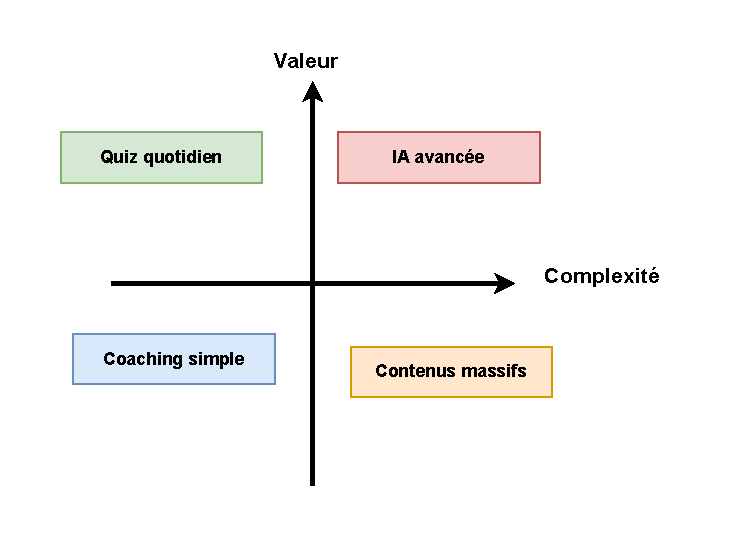
\includegraphics[width=\textwidth,height=0.54\textheight,keepaspectratio]{figures/ipf/priorisation_perimetre.pdf}%
  \or
    % Architecture générale Flutter / React / Supabase / RevenueCat.
    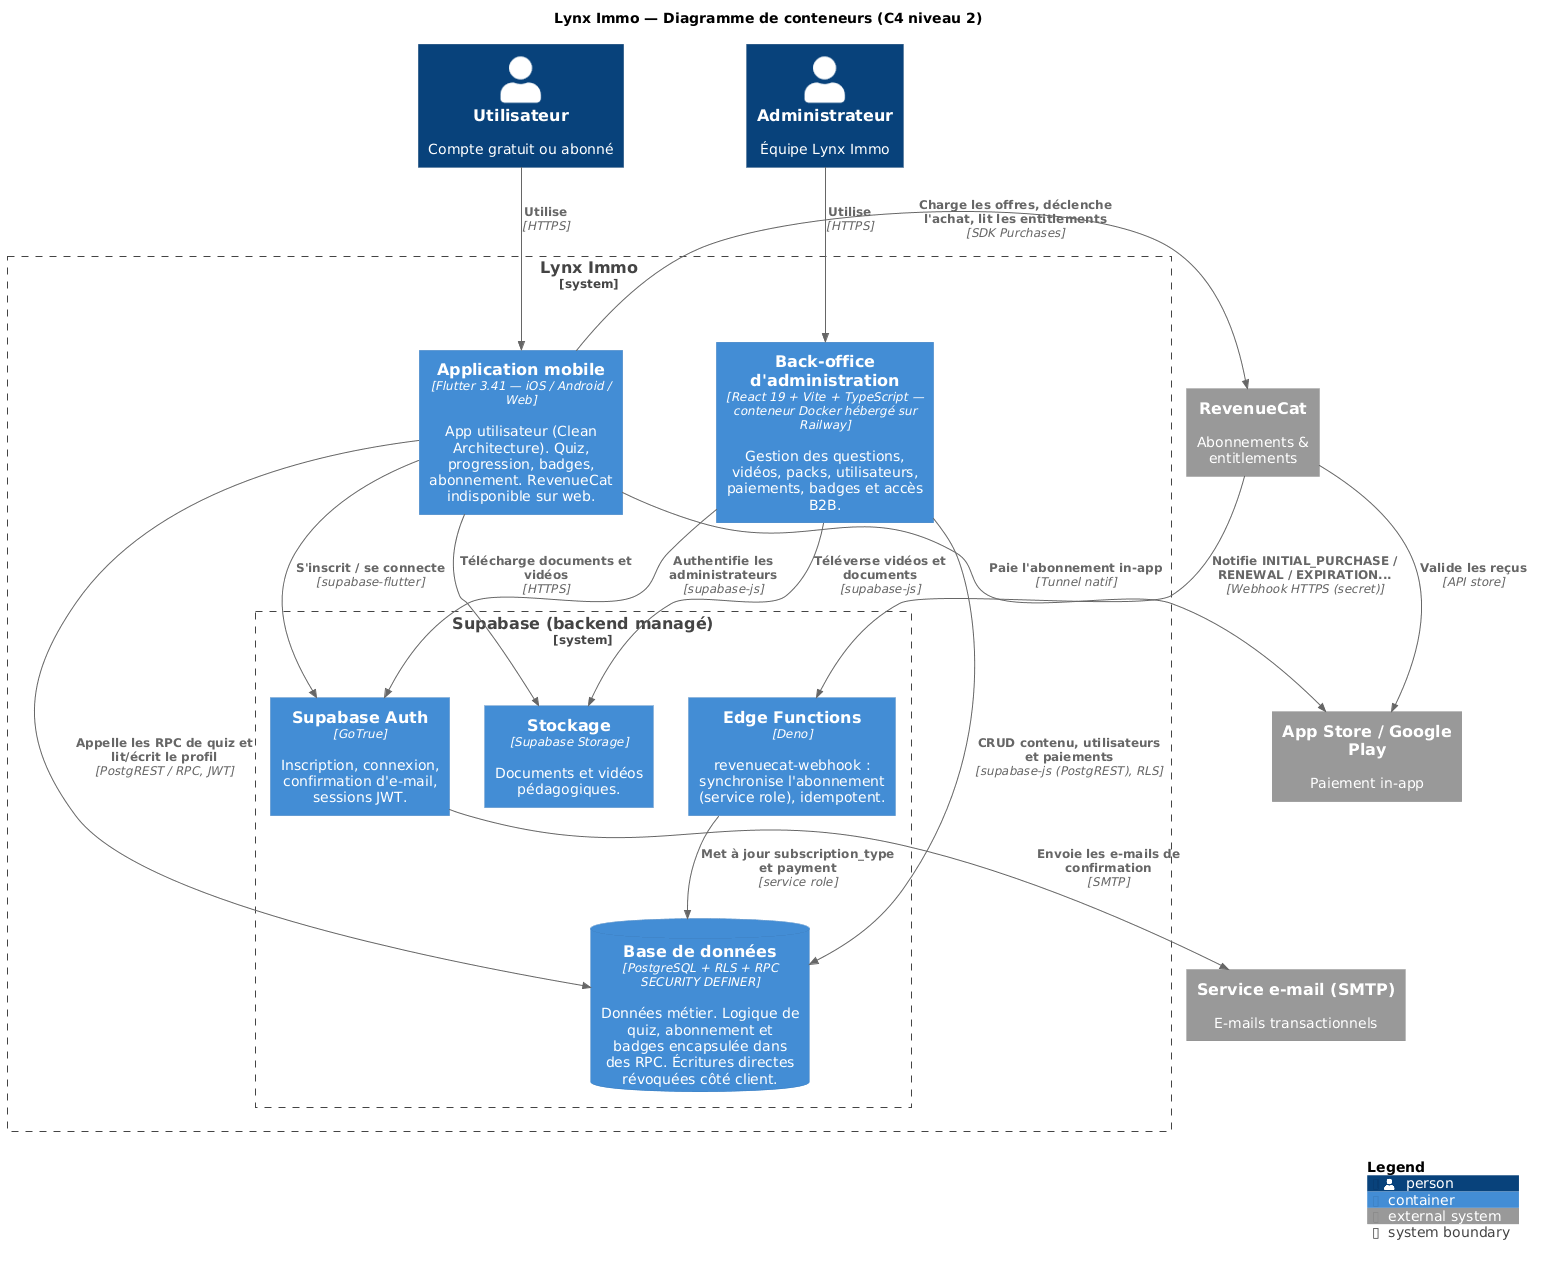
\includegraphics[width=\textwidth,height=0.56\textheight,keepaspectratio]{figures/ipf/architecture.png}%
  \or
    % Principaux écrans mobiles et modules d'administration.
    \begin{minipage}{\textwidth}
      \centering
      \begin{minipage}[t]{0.18\textwidth}
        \centering
        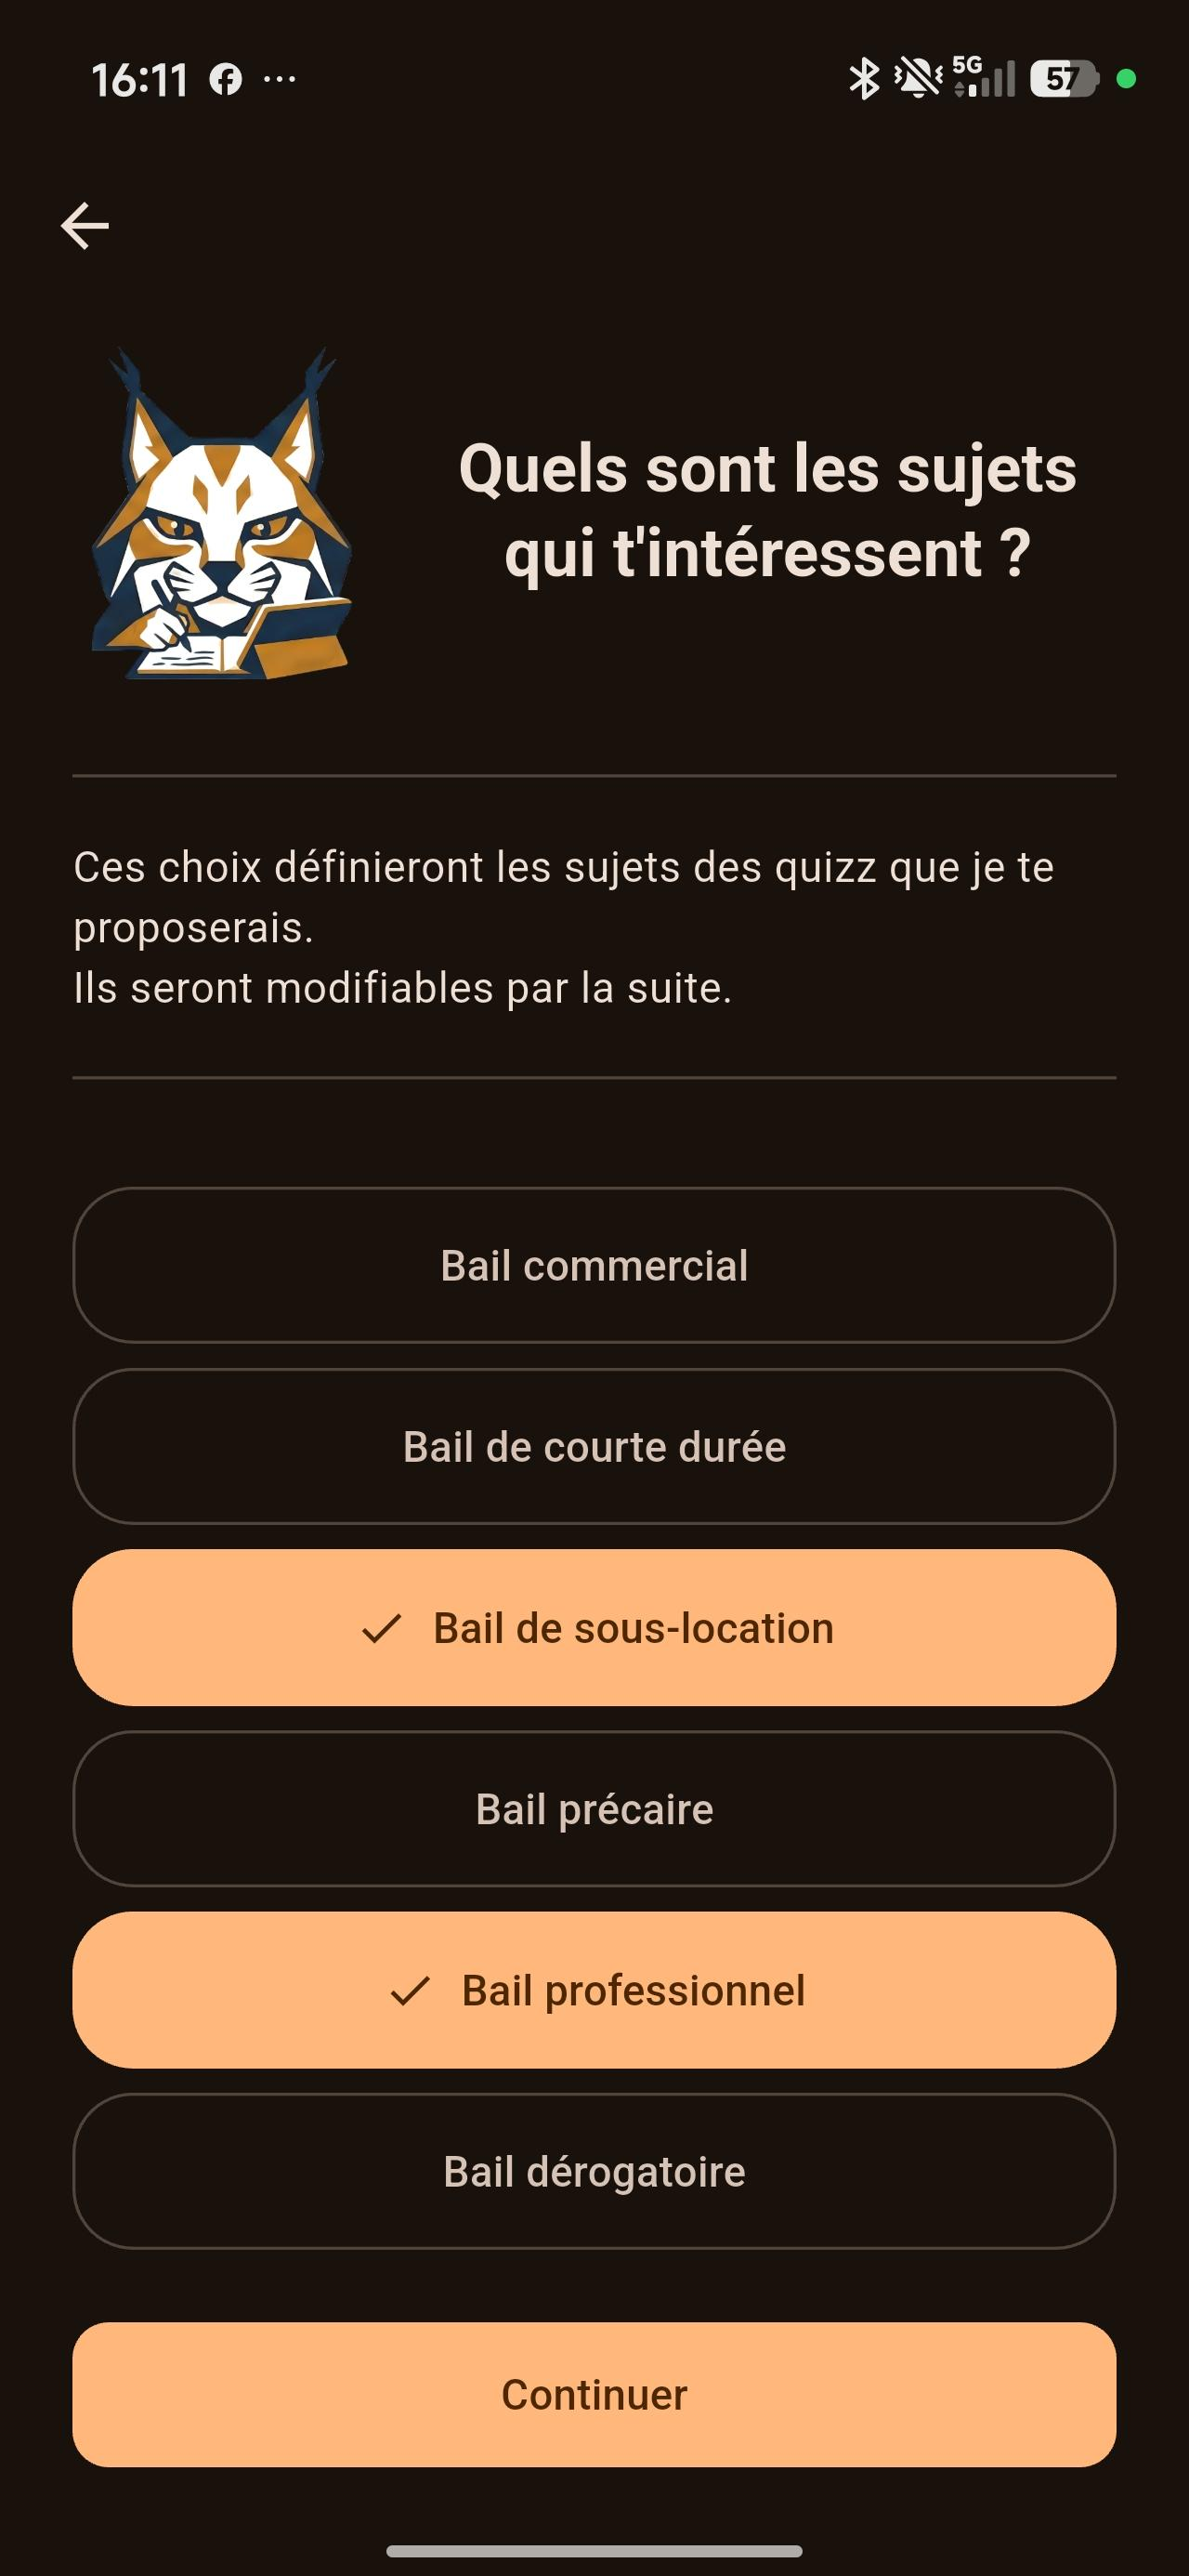
\includegraphics[width=\textwidth,height=0.25\textheight,keepaspectratio]{figures/ipf/onboarding.jpg}\\[-0.05cm]
        {\footnotesize (a) Onboarding}
      \end{minipage}%
      \hfill
      \begin{minipage}[t]{0.18\textwidth}
        \centering
        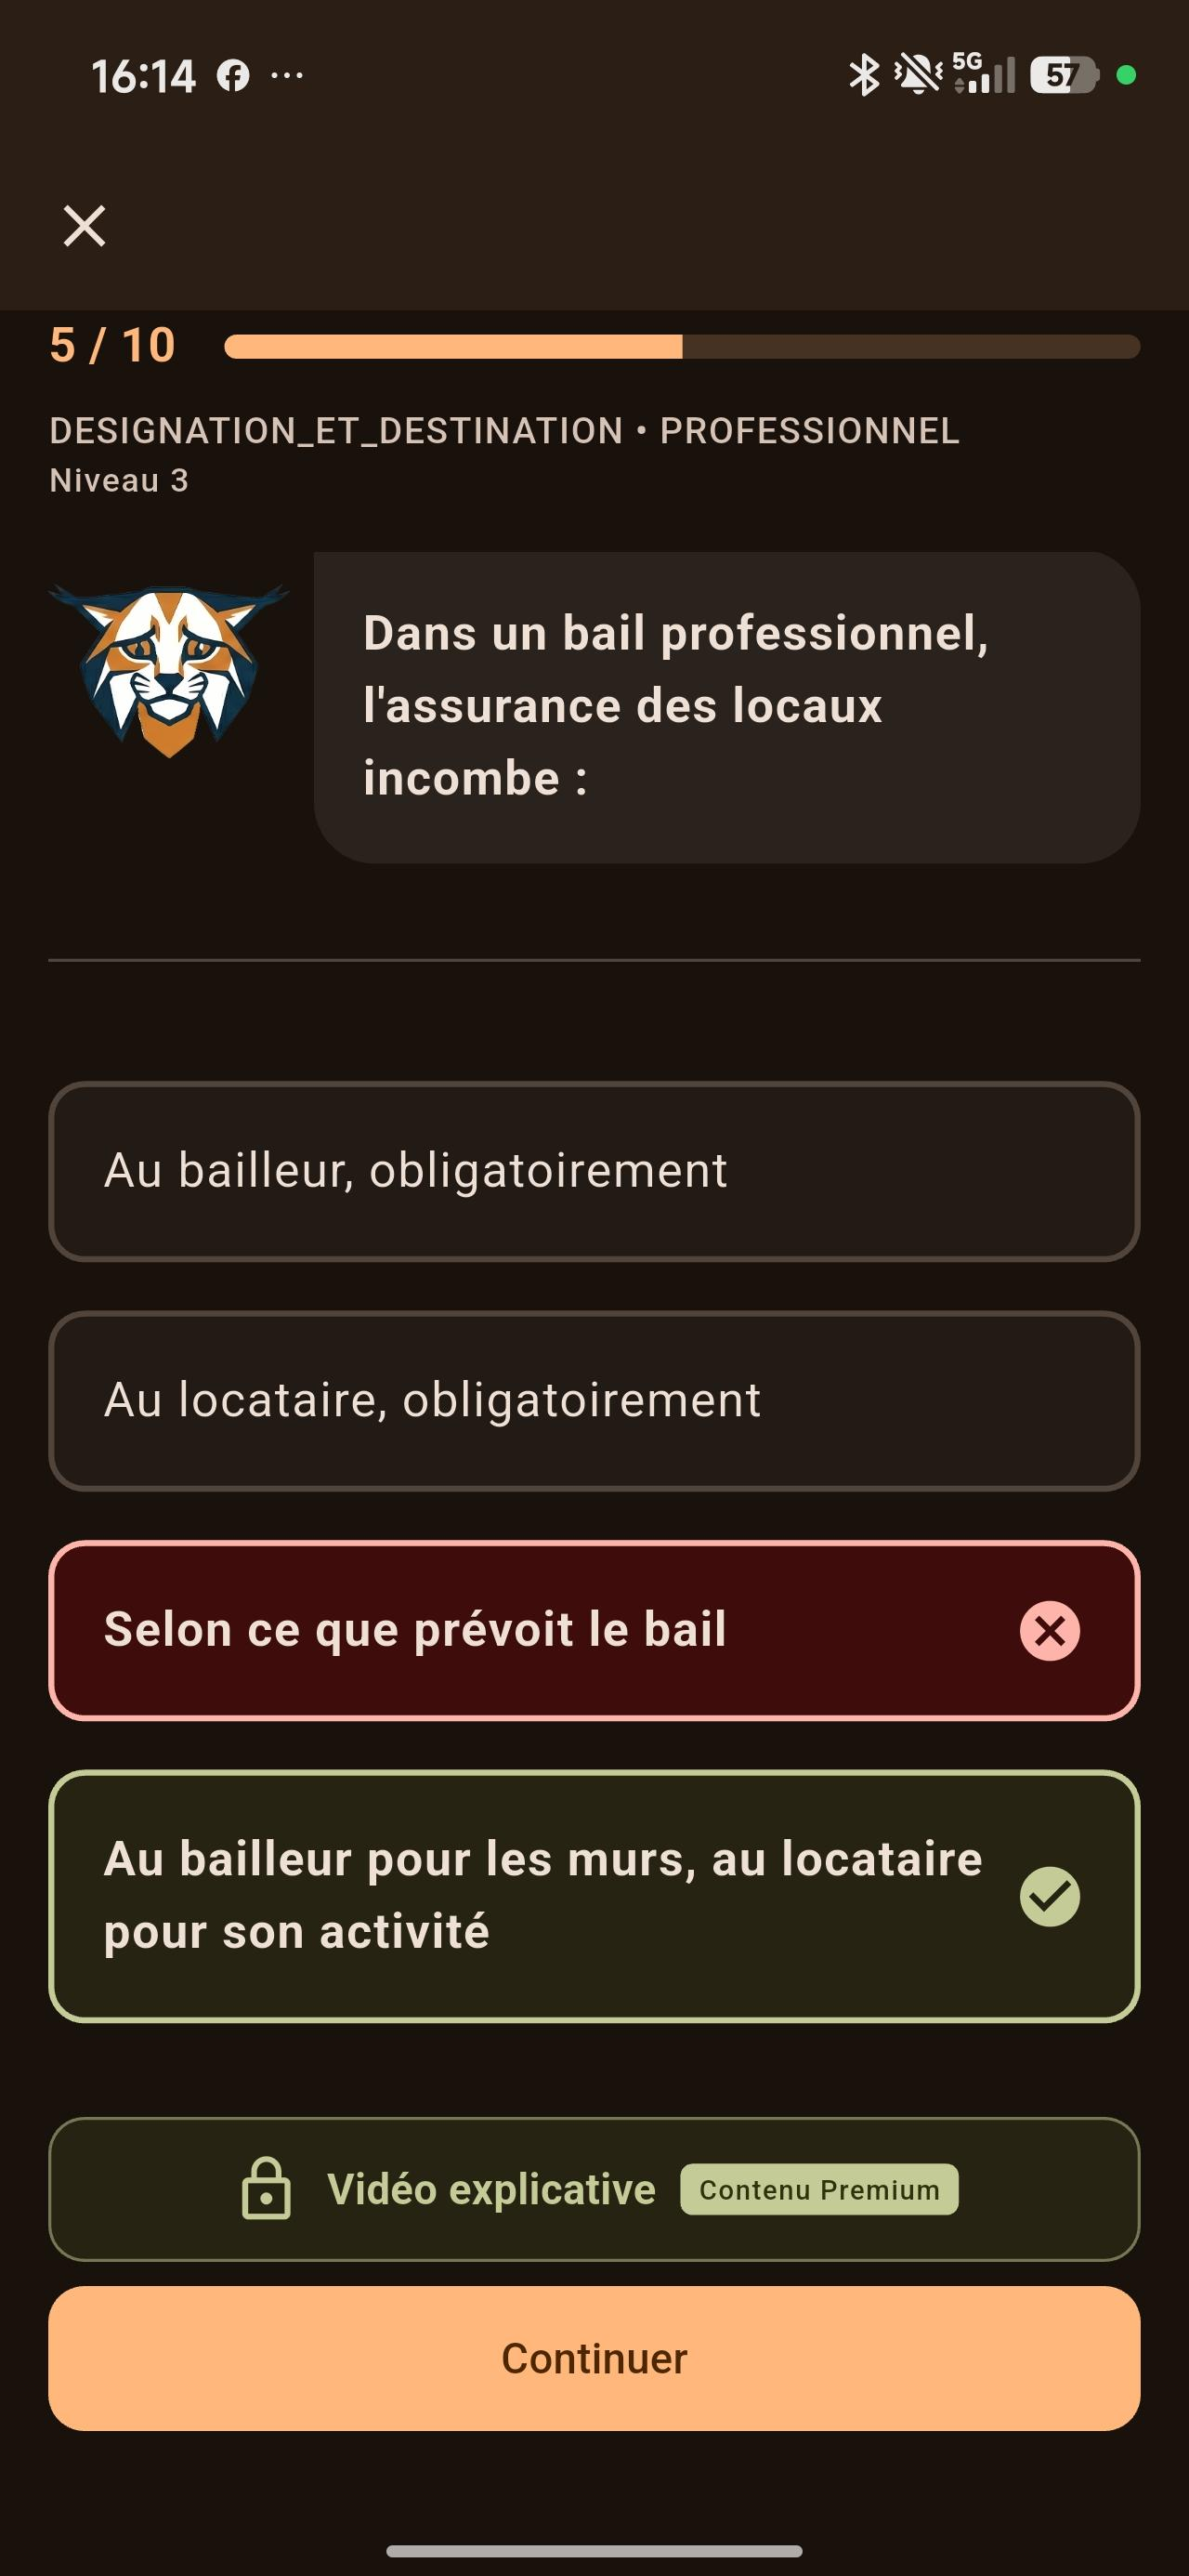
\includegraphics[width=\textwidth,height=0.25\textheight,keepaspectratio]{figures/ipf/quiz.jpg}\\[-0.05cm]
        {\footnotesize (b) Quiz quotidien}
      \end{minipage}%
      \hfill
      \begin{minipage}[t]{0.18\textwidth}
        \centering
        
\includegraphics[width=\textwidth,height=0.25\textheight,keepaspectratio]{figures/ipf/resultat.jpg}\\[-0.05cm]
        {\footnotesize (c) Résultat}
      \end{minipage}%
      \hfill
      \begin{minipage}[t]{0.18\textwidth}
        \centering
        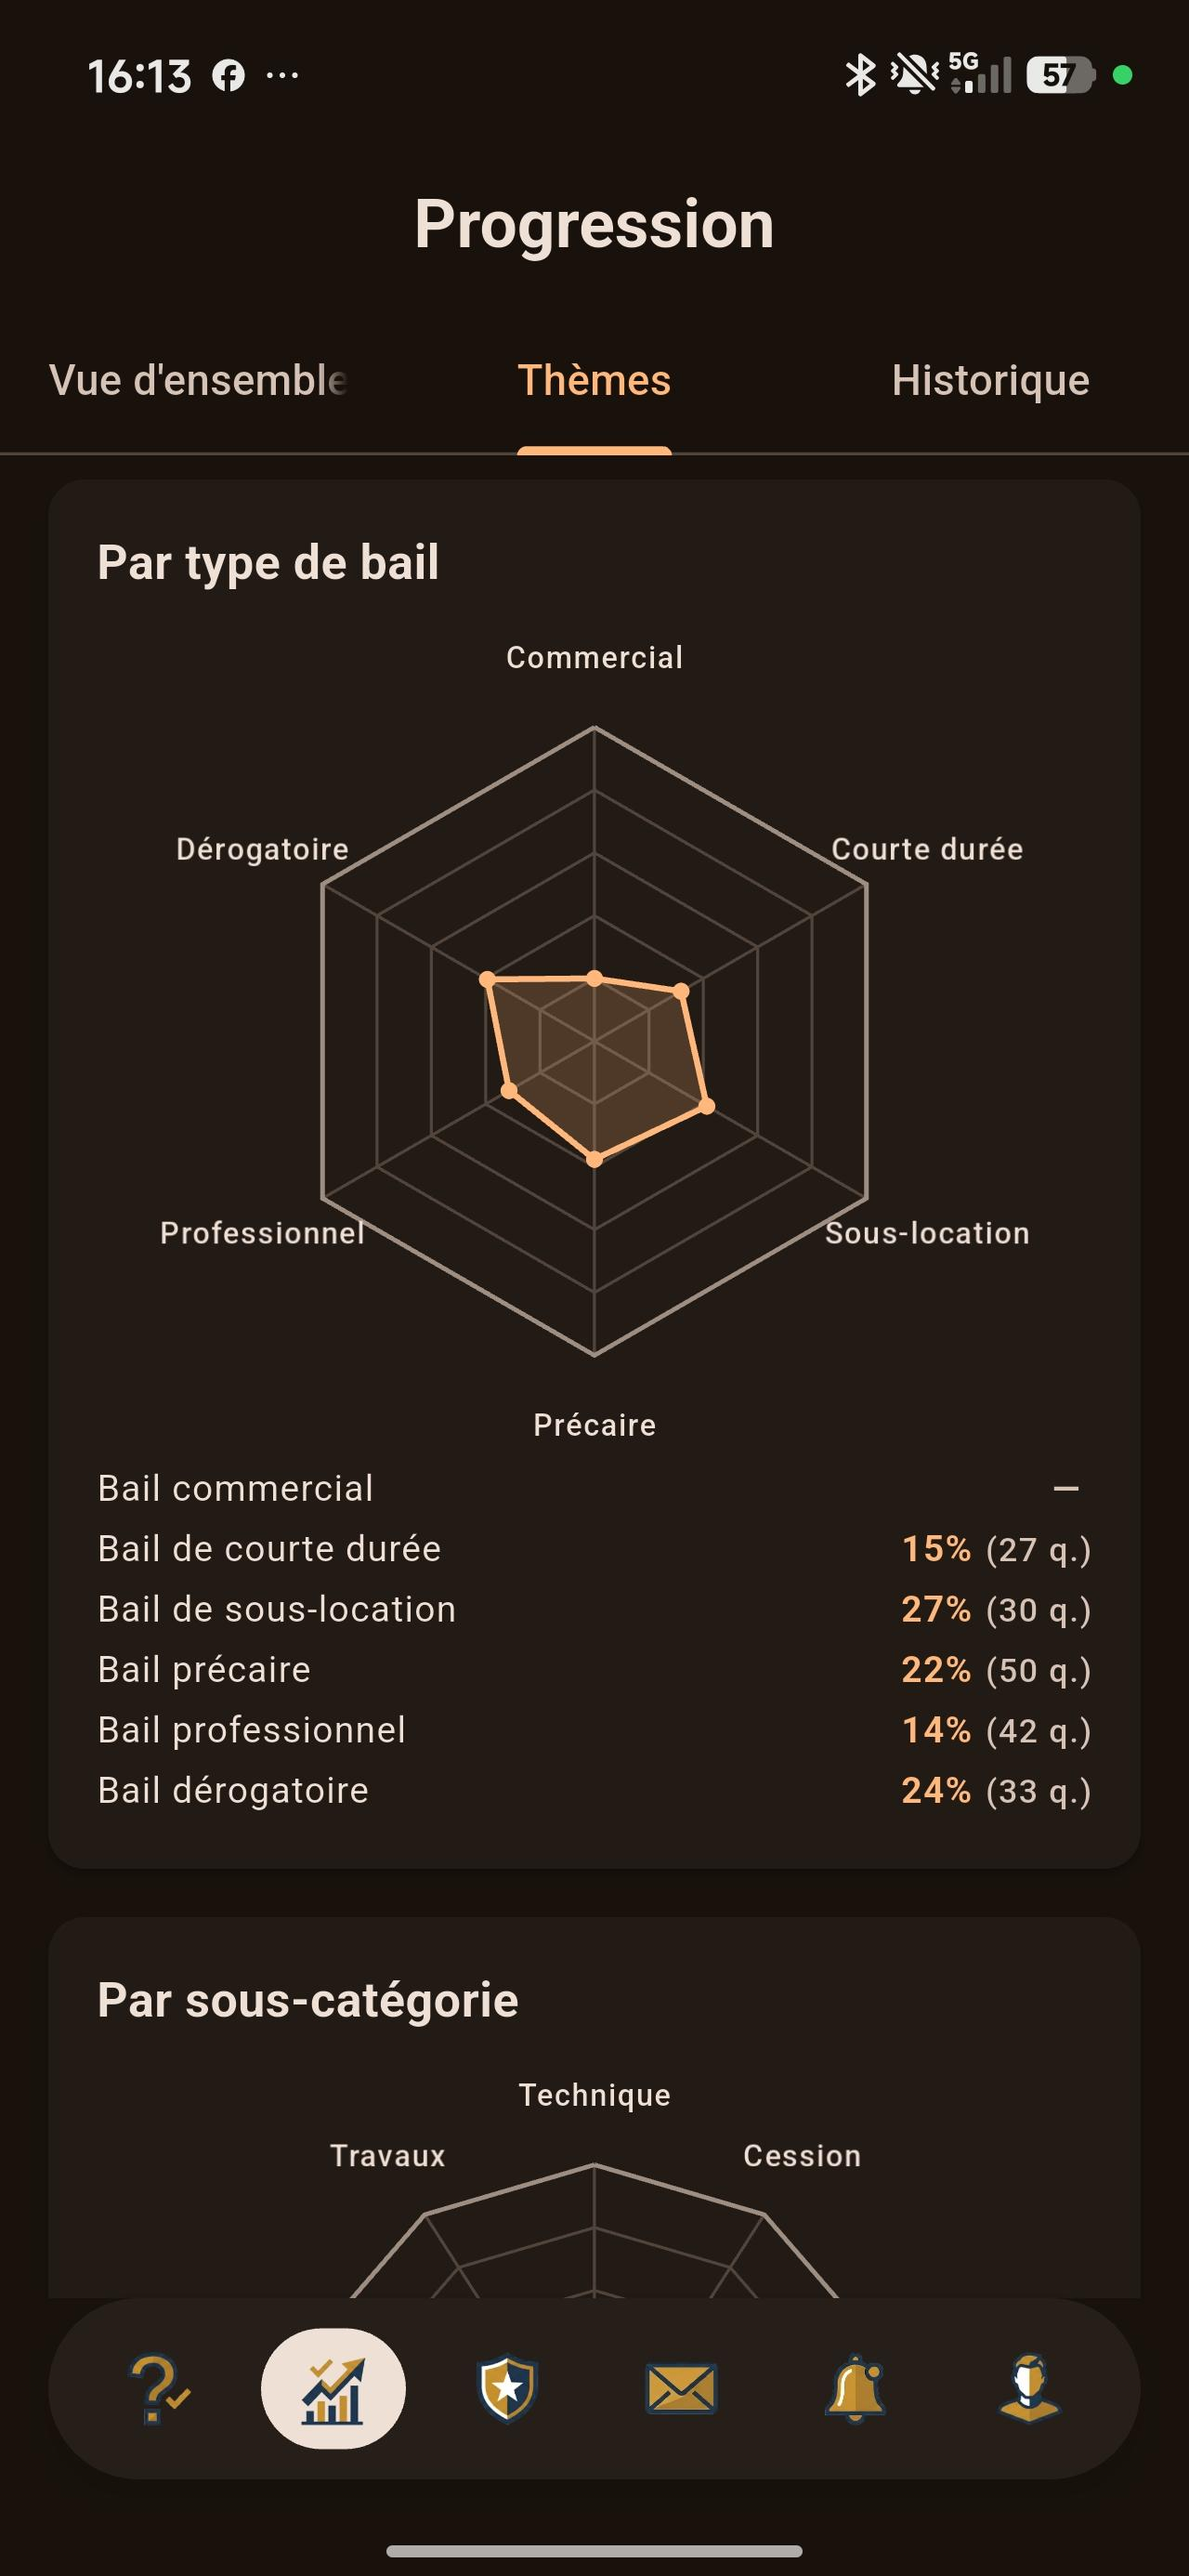
\includegraphics[width=\textwidth,height=0.25\textheight,keepaspectratio]{figures/ipf/progression.jpg}\\[-0.05cm]
        {\footnotesize (d) Progression}
      \end{minipage}%
      \hfill
      \begin{minipage}[t]{0.18\textwidth}
        \centering
        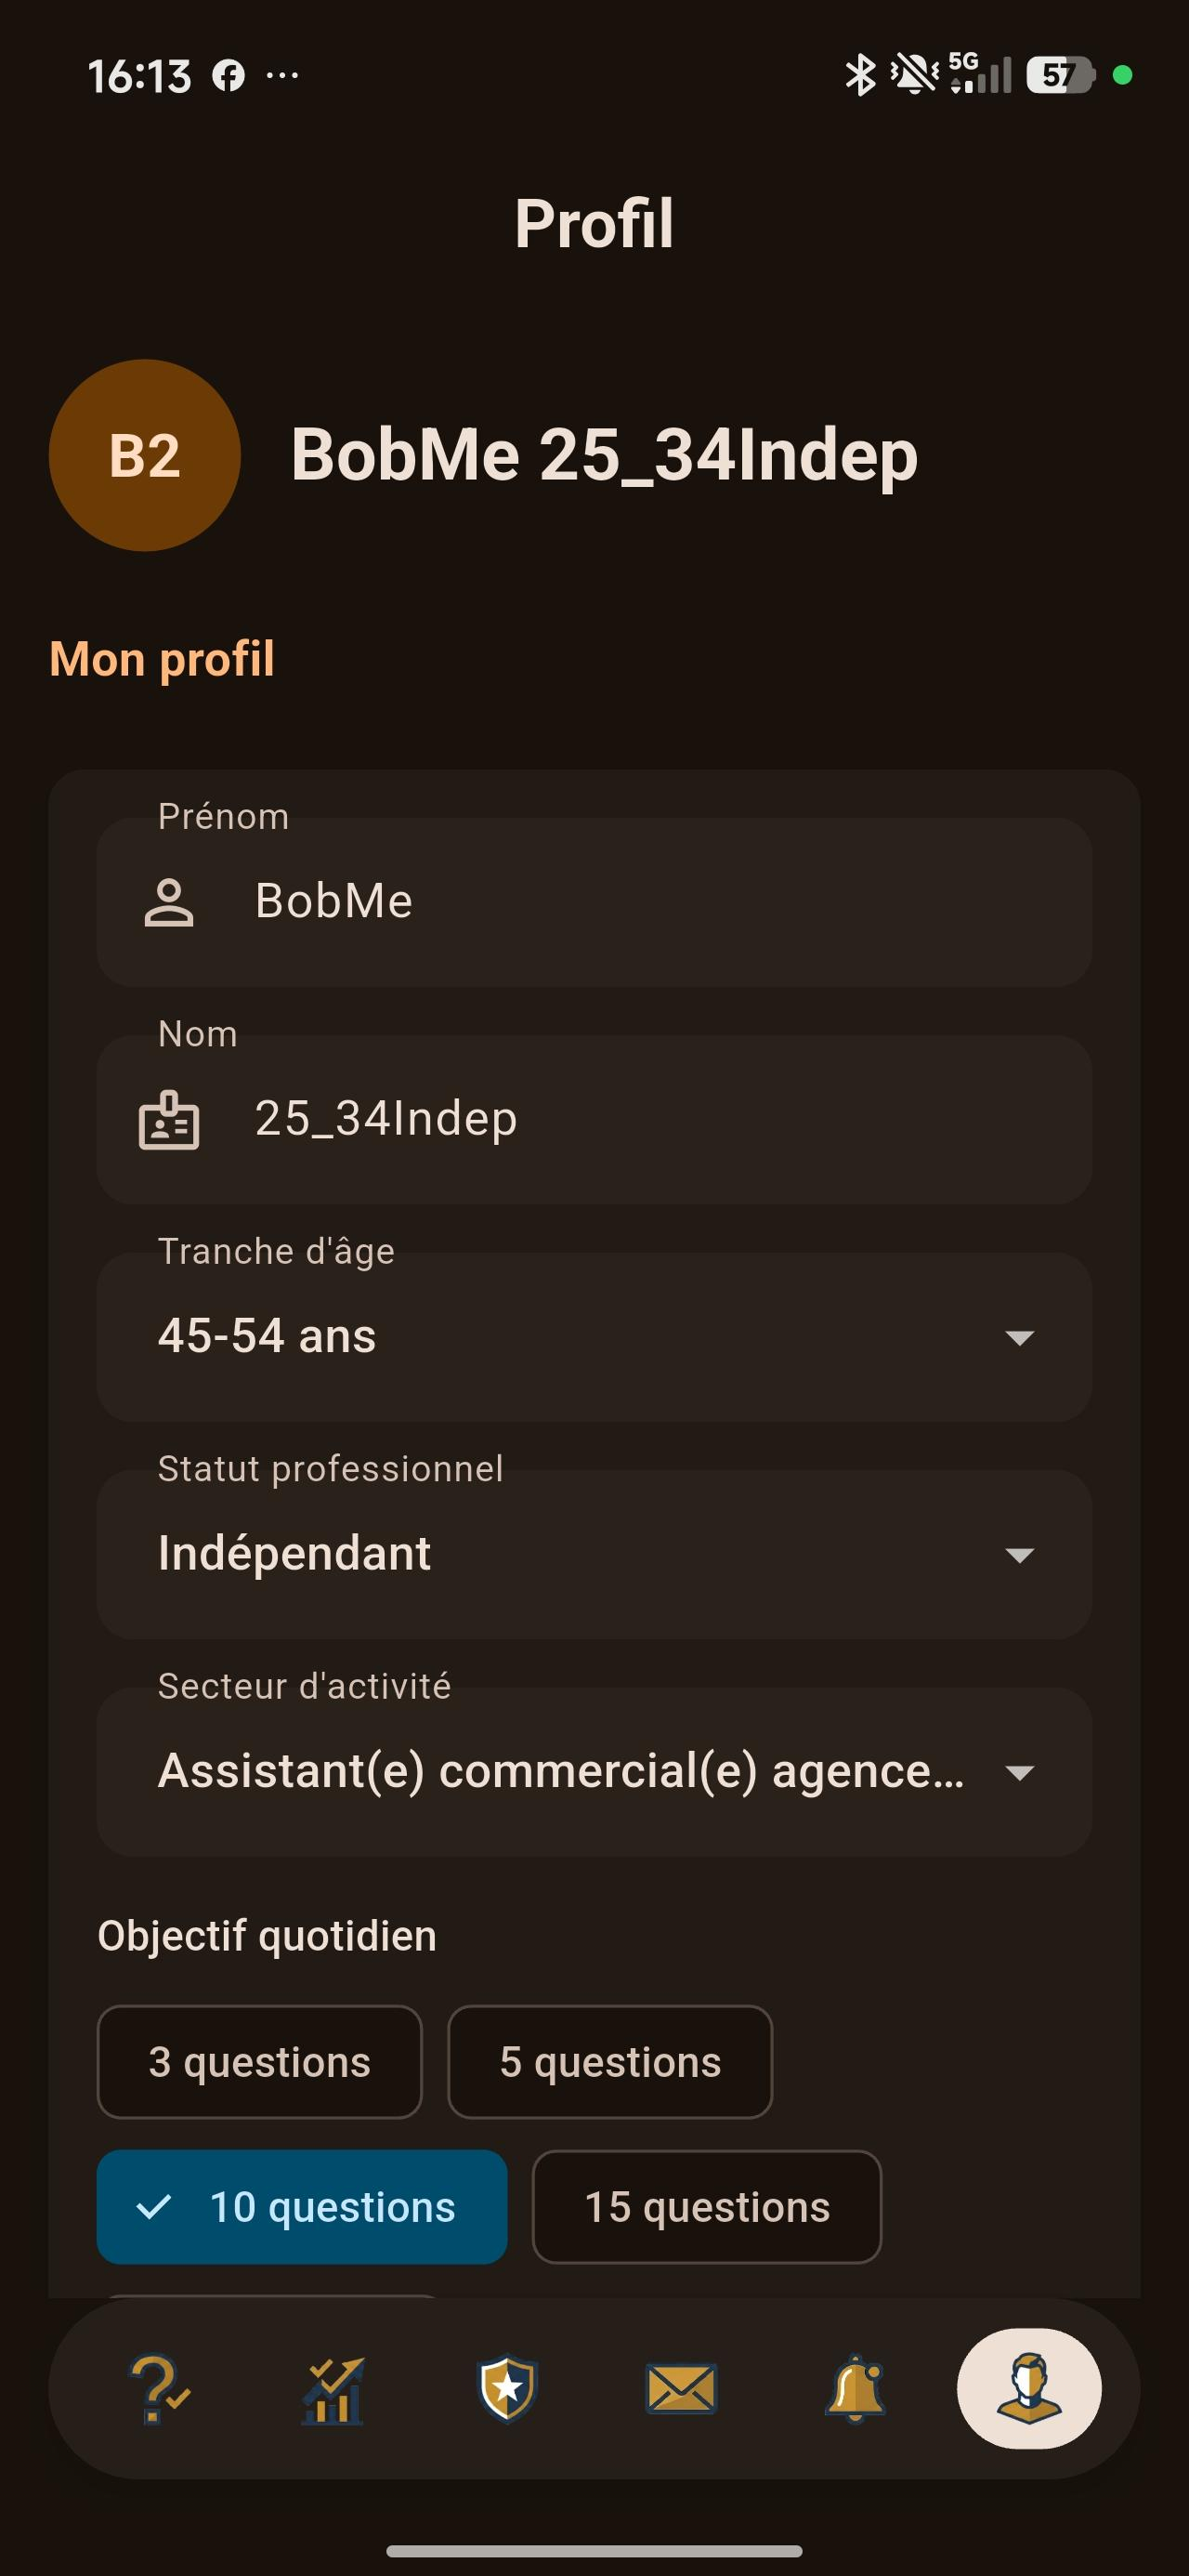
\includegraphics[width=\textwidth,height=0.25\textheight,keepaspectratio]{figures/ipf/profil.jpg}\\[-0.05cm]
        {\footnotesize (e) Profil}
      \end{minipage}

      \vspace{0.25cm}

      \begin{minipage}[t]{0.31\textwidth}
        \centering
        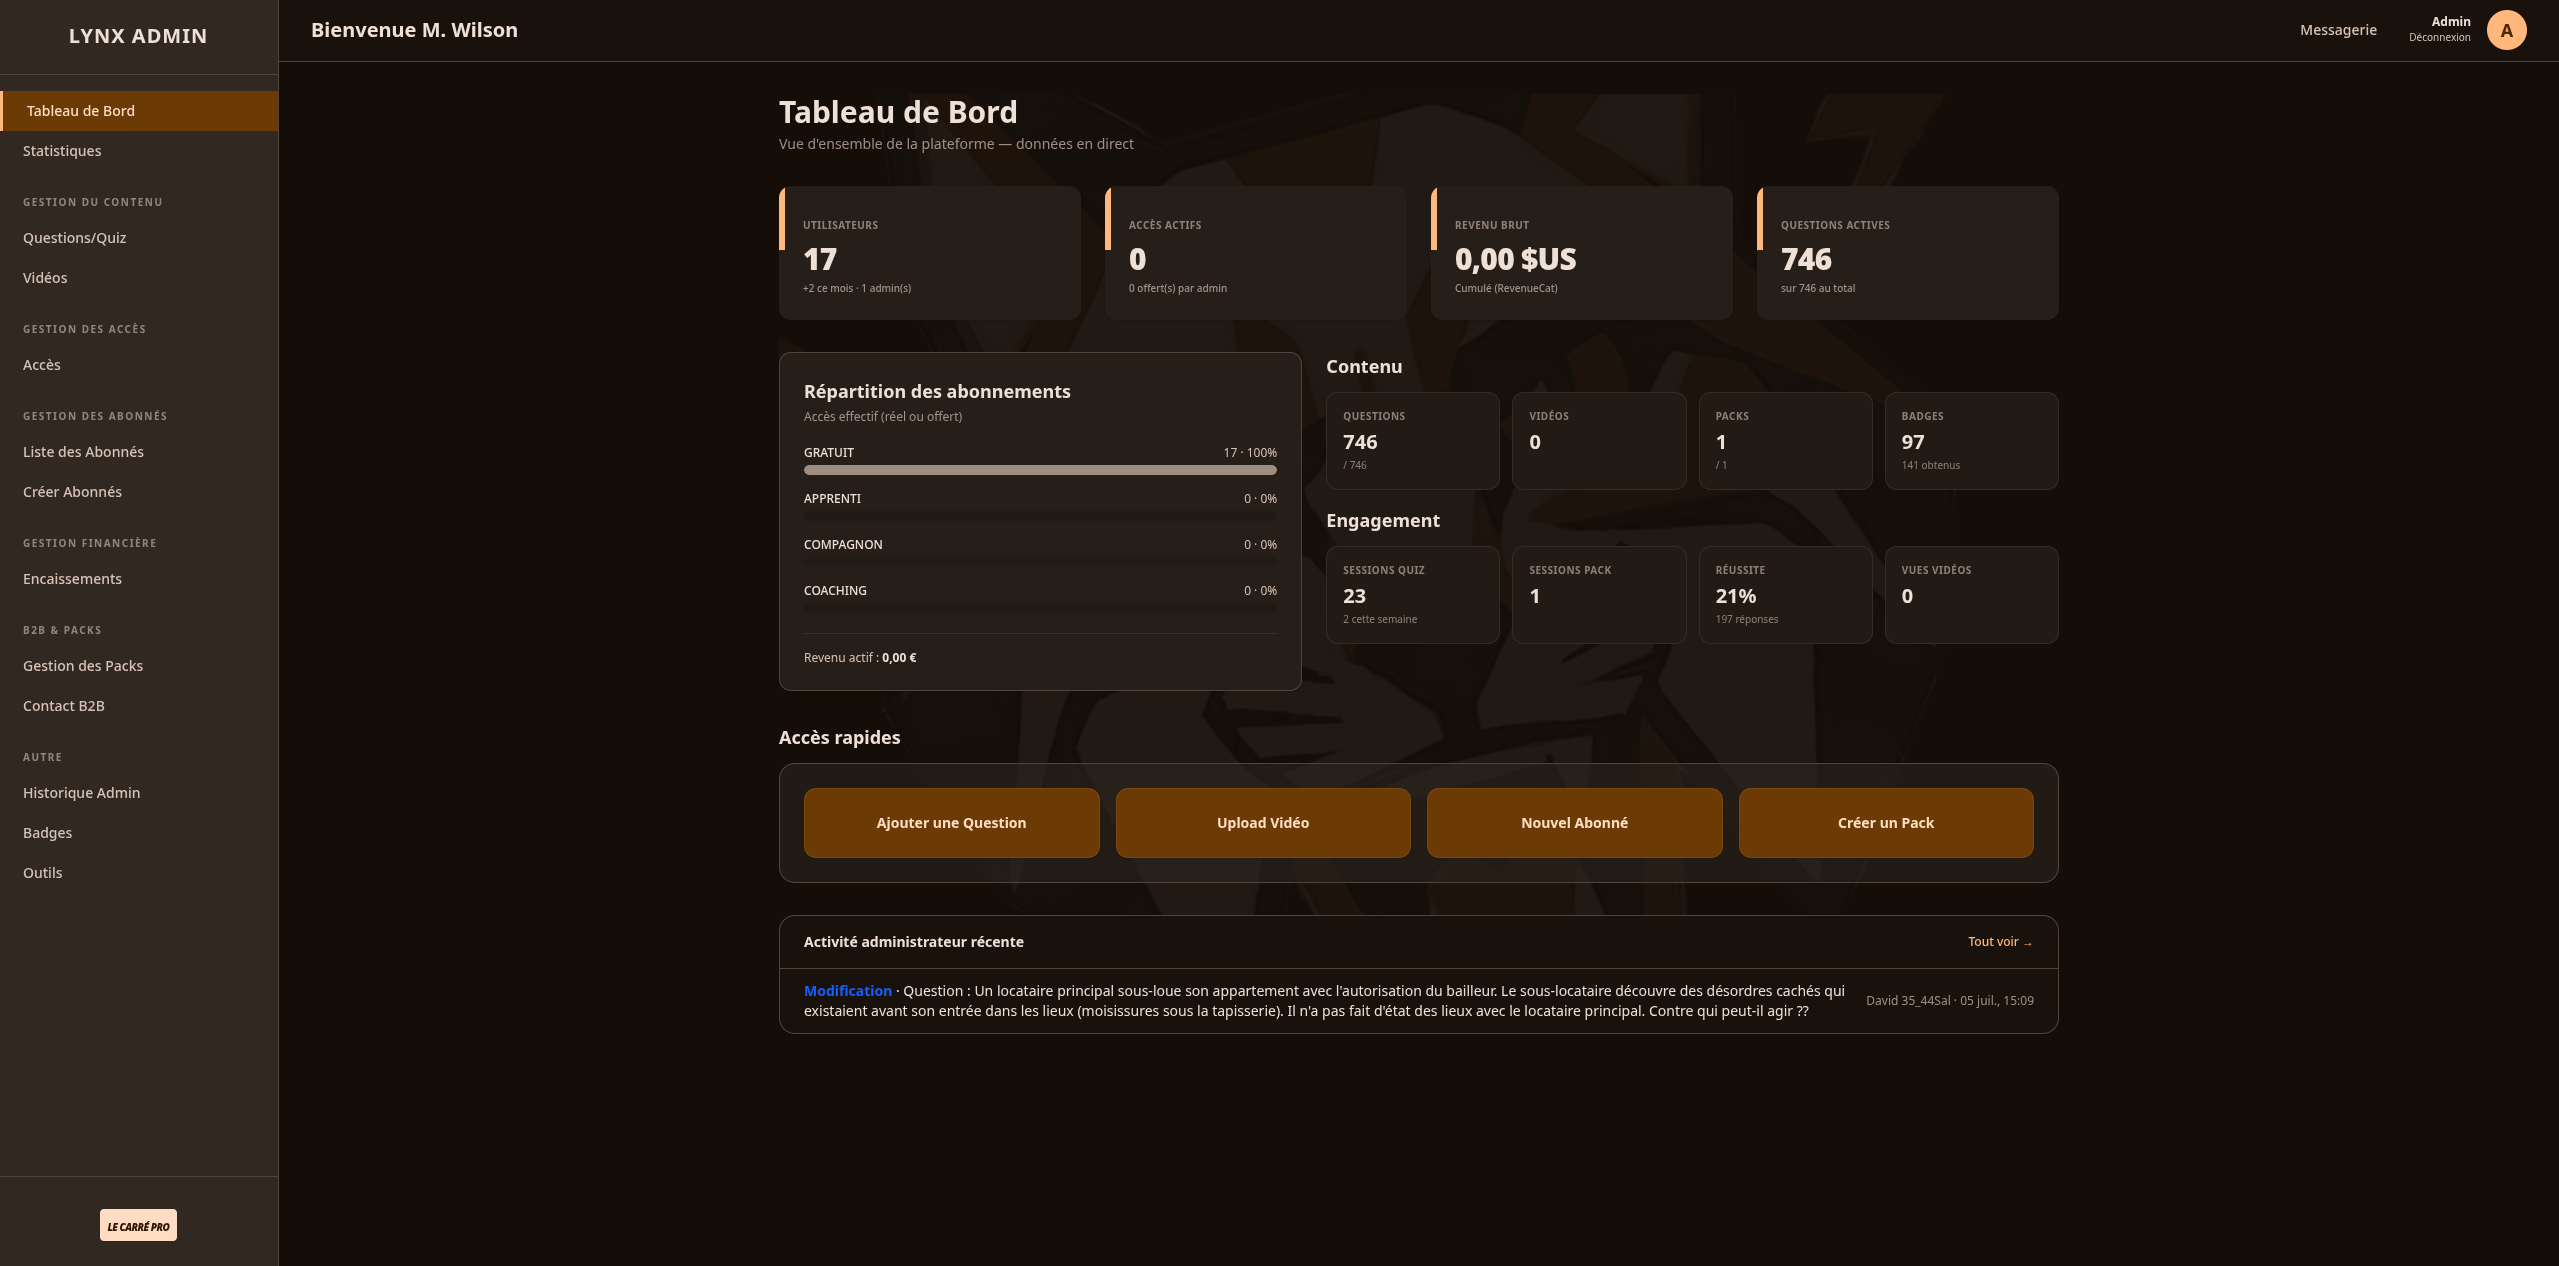
\includegraphics[width=\textwidth,height=0.18\textheight,keepaspectratio]{figures/ipf/tableau_bord_admin.png}\\[-0.05cm]
        {\footnotesize (f) Tableau de bord}
      \end{minipage}%
      \hfill
      \begin{minipage}[t]{0.31\textwidth}
        \centering
        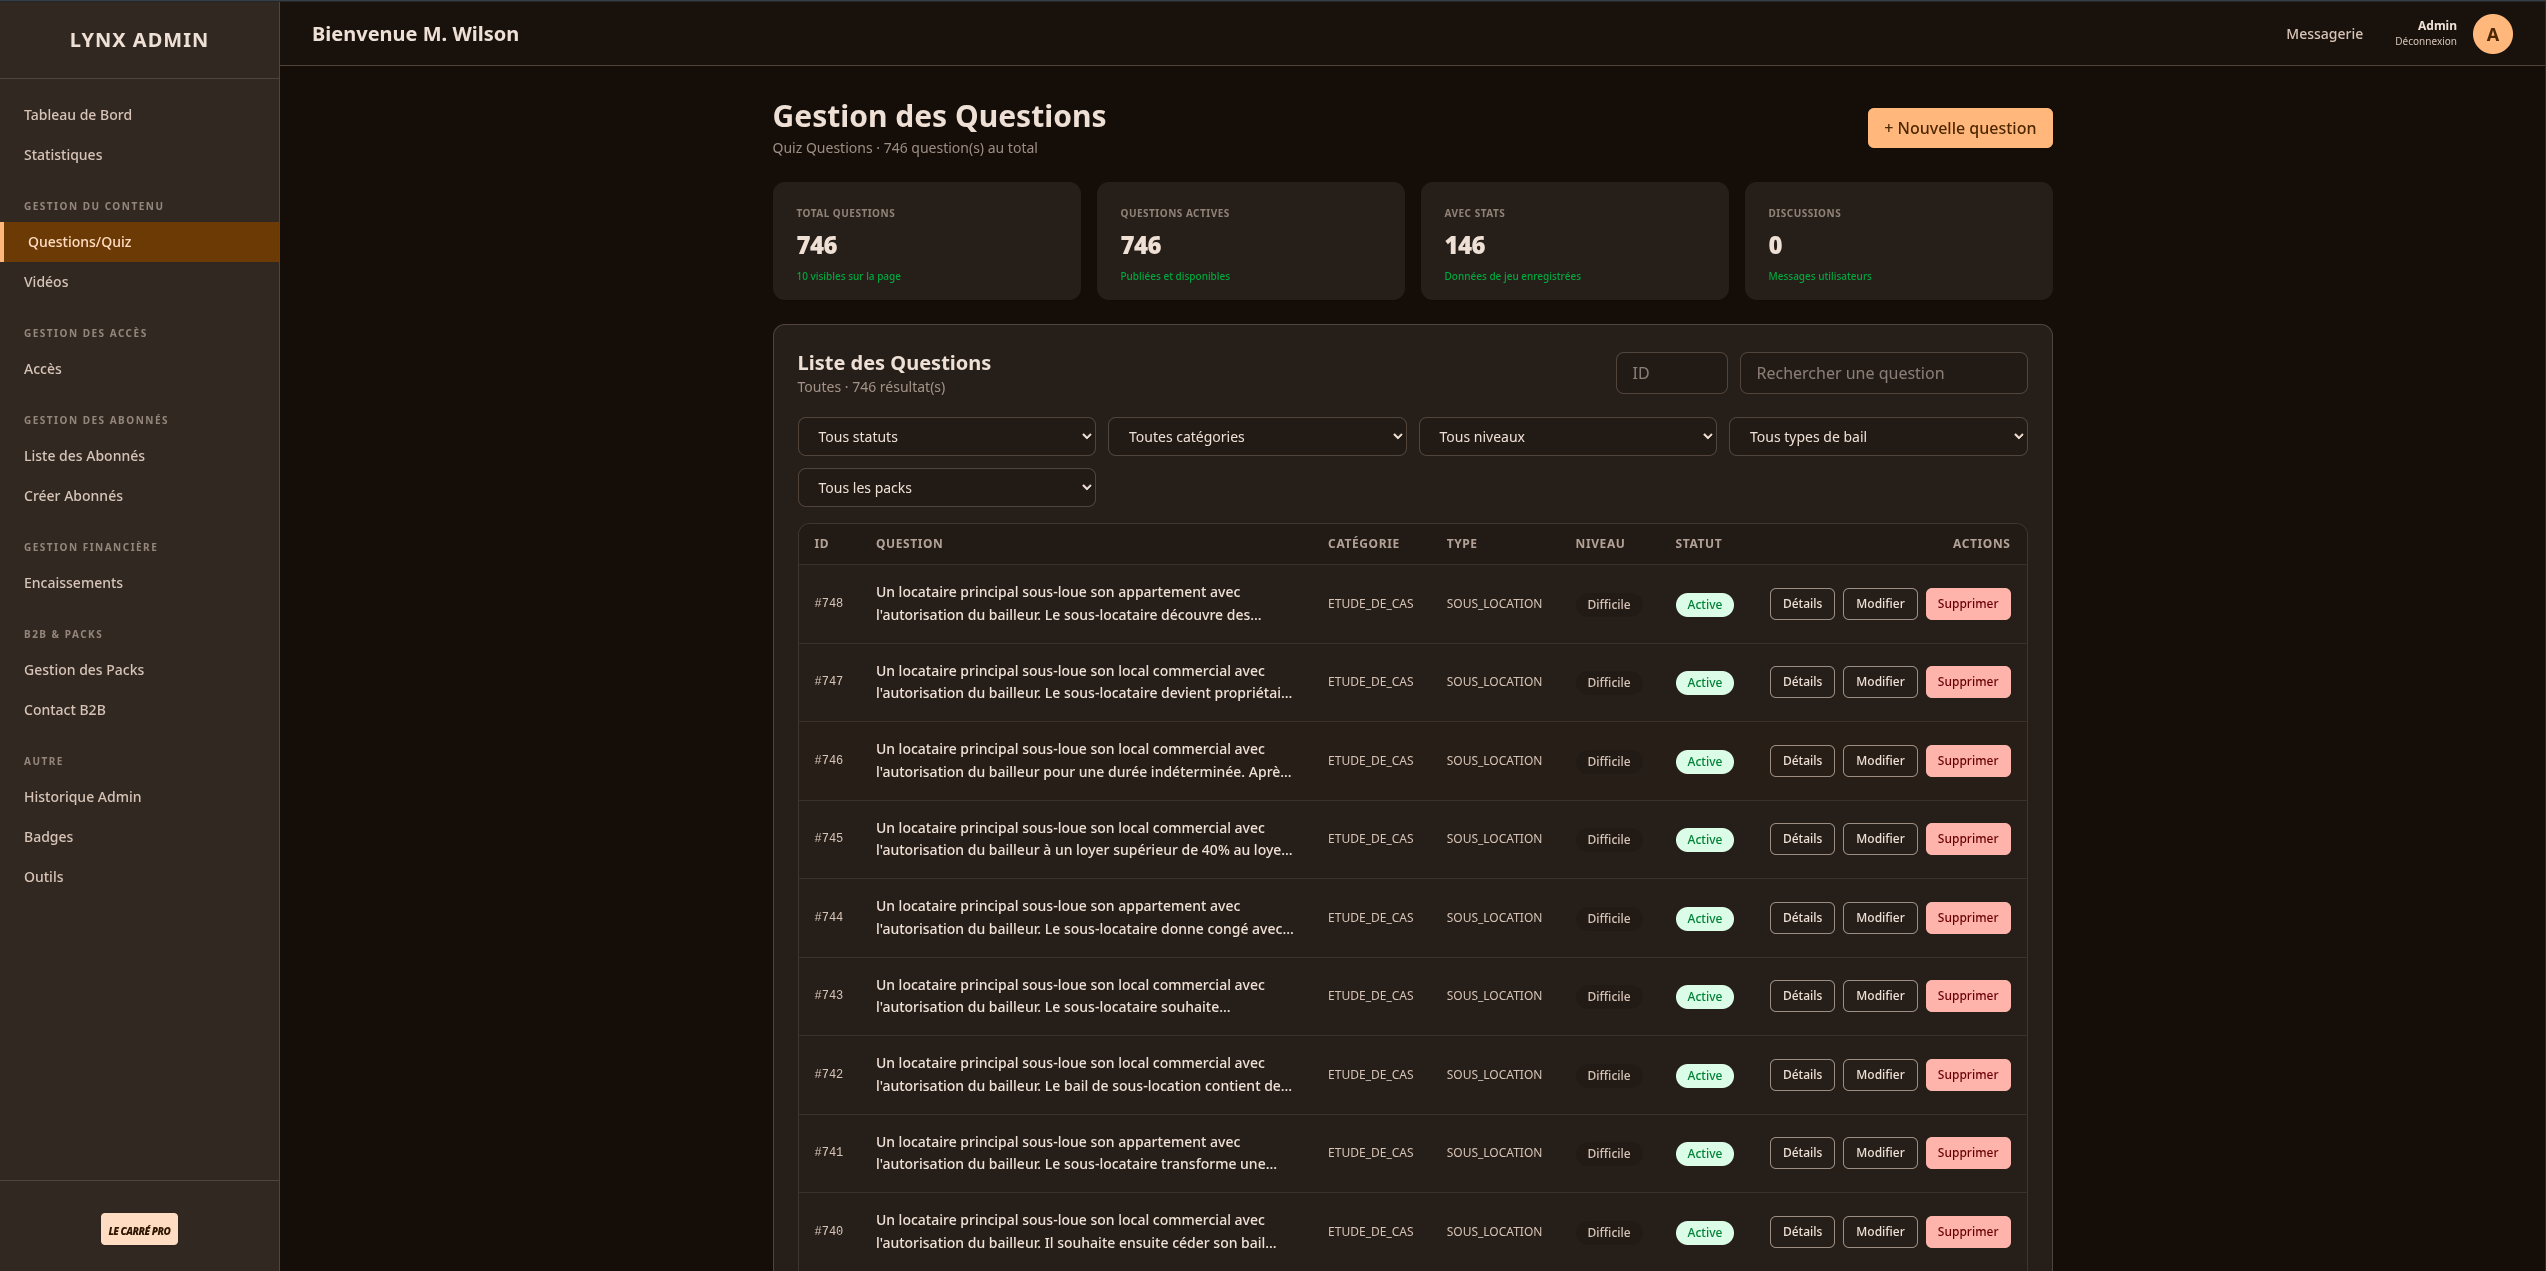
\includegraphics[width=\textwidth,height=0.18\textheight,keepaspectratio]{figures/ipf/admin_questions.png}\\[-0.05cm]
        {\footnotesize (g) Gestion des questions}
      \end{minipage}%
      \hfill
      \begin{minipage}[t]{0.31\textwidth}
        \centering
        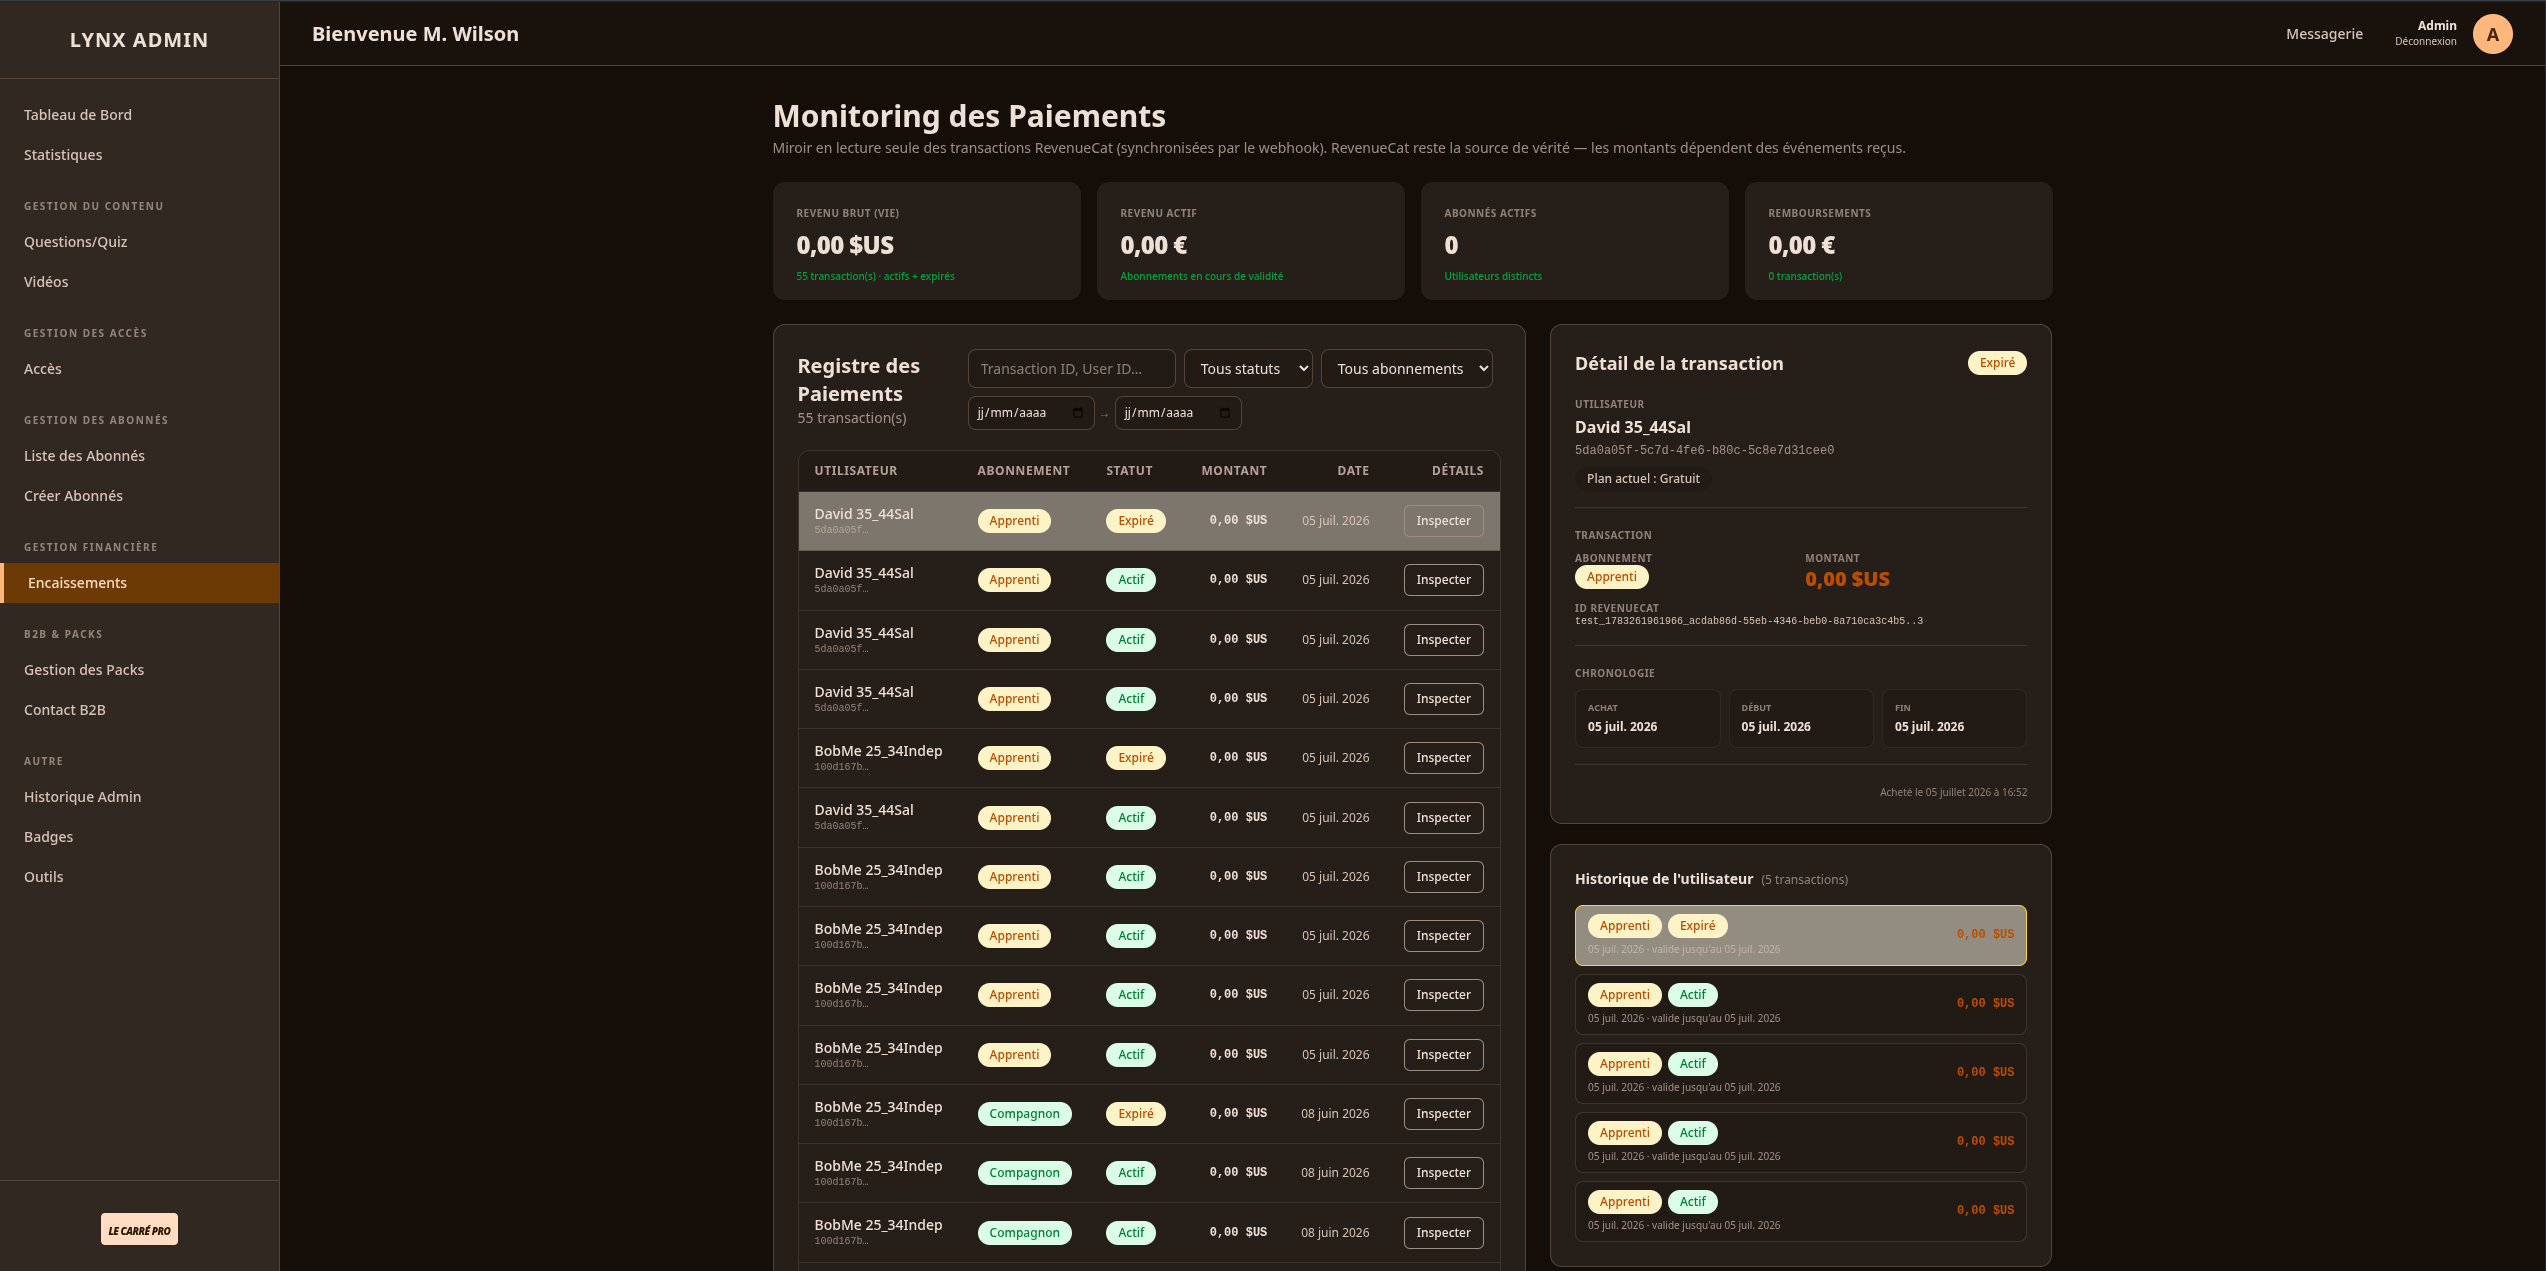
\includegraphics[width=\textwidth,height=0.18\textheight,keepaspectratio]{figures/ipf/admin_encaissement.png}\\[-0.05cm]
        {\footnotesize (h) Encaissements}
      \end{minipage}
    \end{minipage}%
  \or
    % Feuille de route et diagramme de Gantt.
    \begin{minipage}{\textwidth}
      \centering
      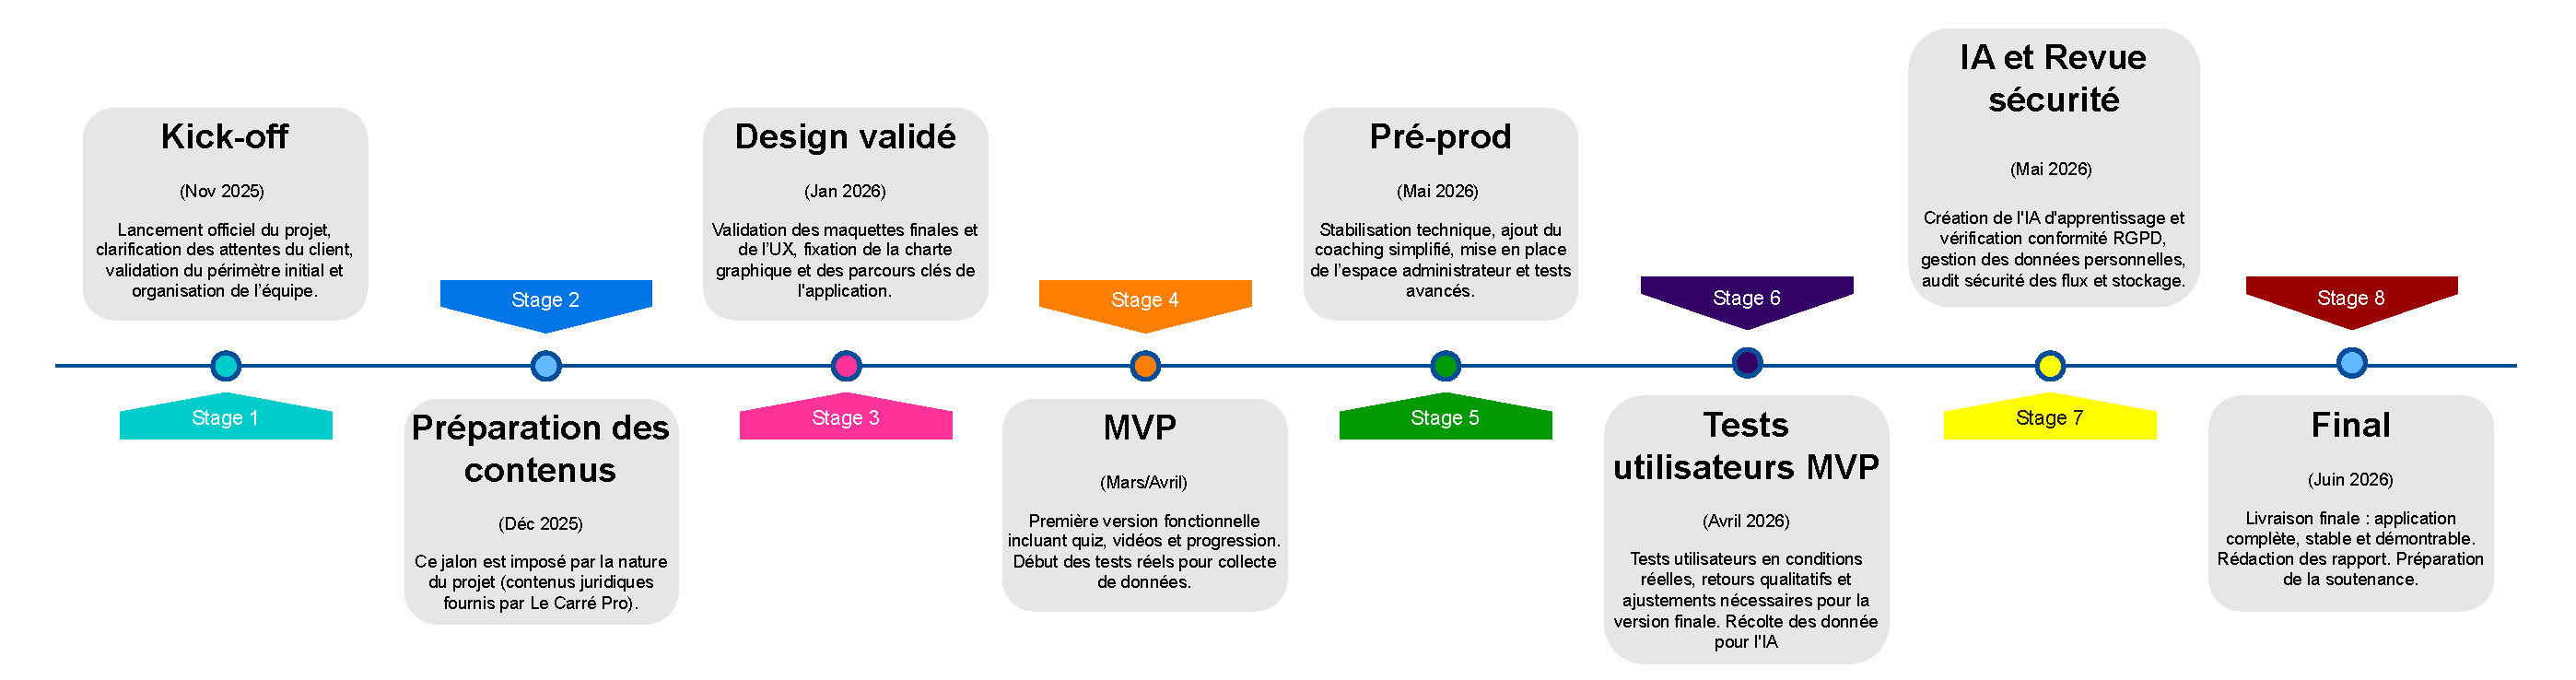
\includegraphics[width=\textwidth,height=0.20\textheight,keepaspectratio]{figures/ipf/roadmap_calendrier.pdf}\\[0.2cm]
      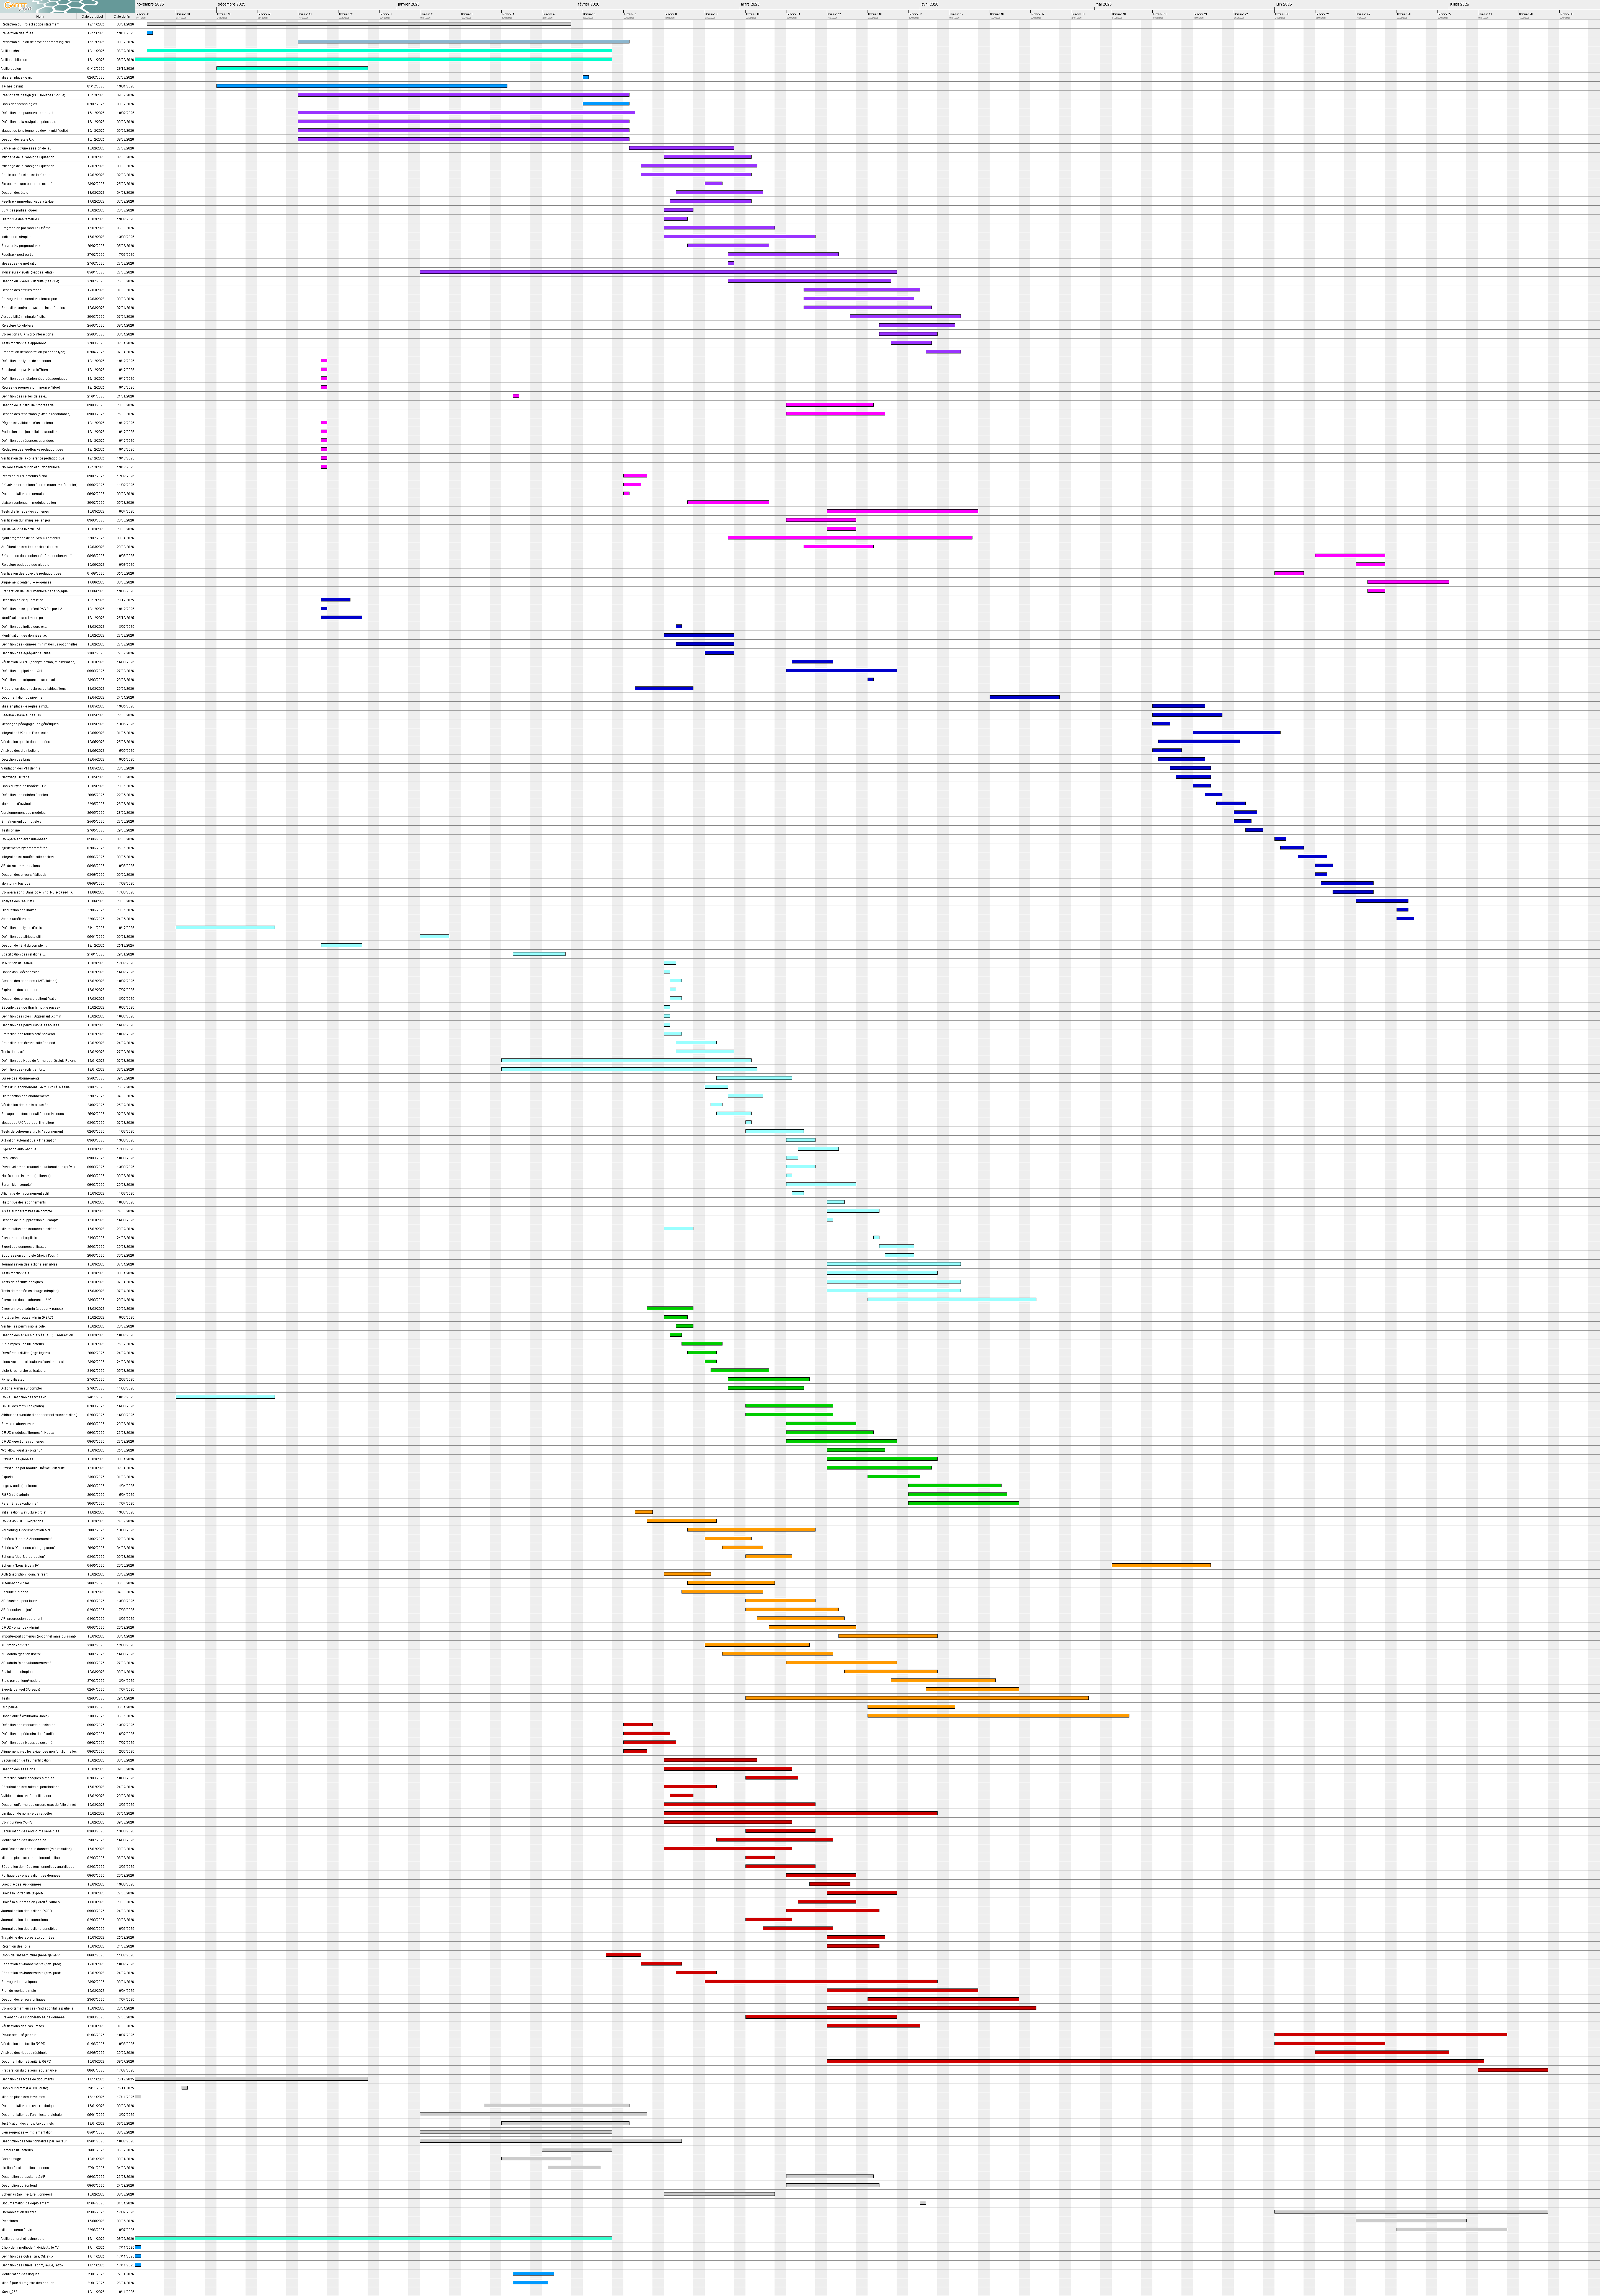
\includegraphics[width=\textwidth,height=0.31\textheight,keepaspectratio]{figures/ipf/gant.png}
    \end{minipage}%
  \or
    % Méthode hybride de conduite du projet.
    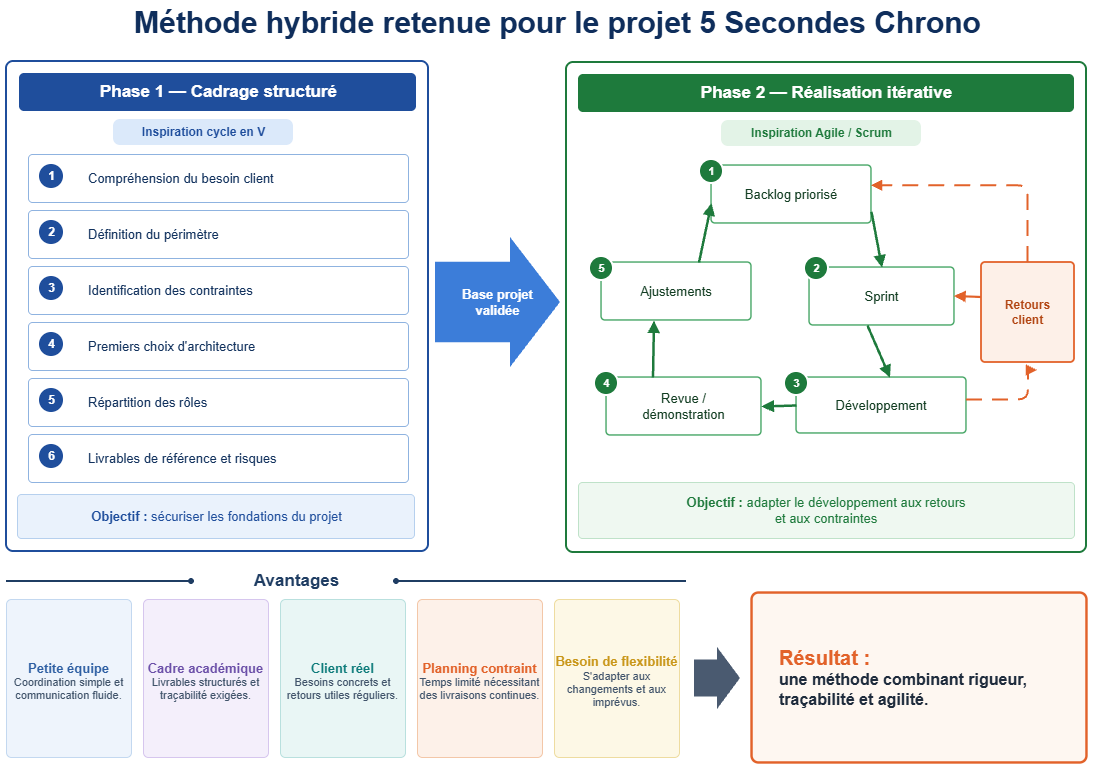
\includegraphics[width=\textwidth,height=0.52\textheight,keepaspectratio]{figures/ipf/methode_hybride_5sc.png}%
  \or
    % Organigramme et répartition des rôles.
    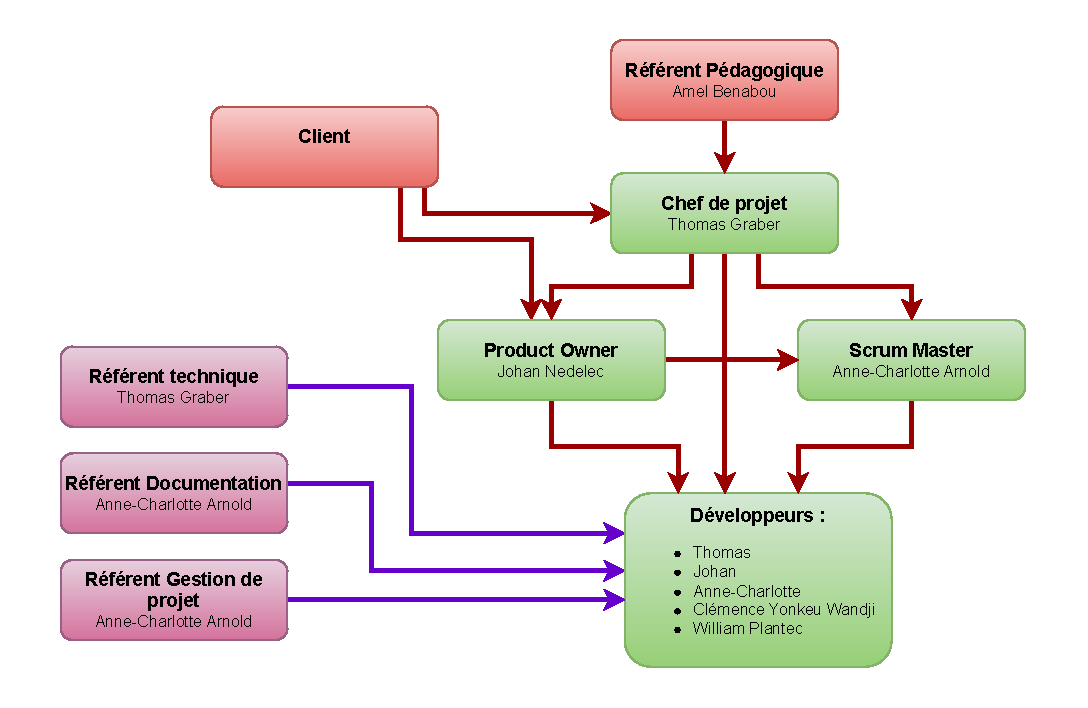
\includegraphics[width=\textwidth,height=0.56\textheight,keepaspectratio]{figures/ipf/organigramme.pdf}%
  \or
    % Vues Jira utilisées pour le pilotage opérationnel.
    \begin{minipage}{\textwidth}
      \centering
      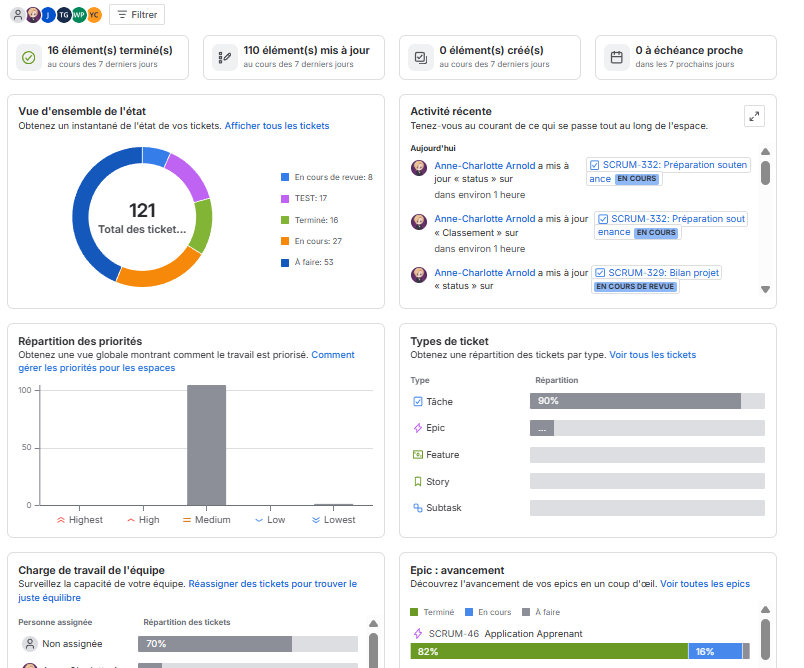
\includegraphics[width=\textwidth,height=0.18\textheight,keepaspectratio]{figures/ipf/vue_synthetique_avancement_jira.png}\\[-0.05cm]
      {\footnotesize (a) Vue synthétique de l'avancement}\\[0.2cm]
      \begin{minipage}[t]{0.49\textwidth}
        \centering
        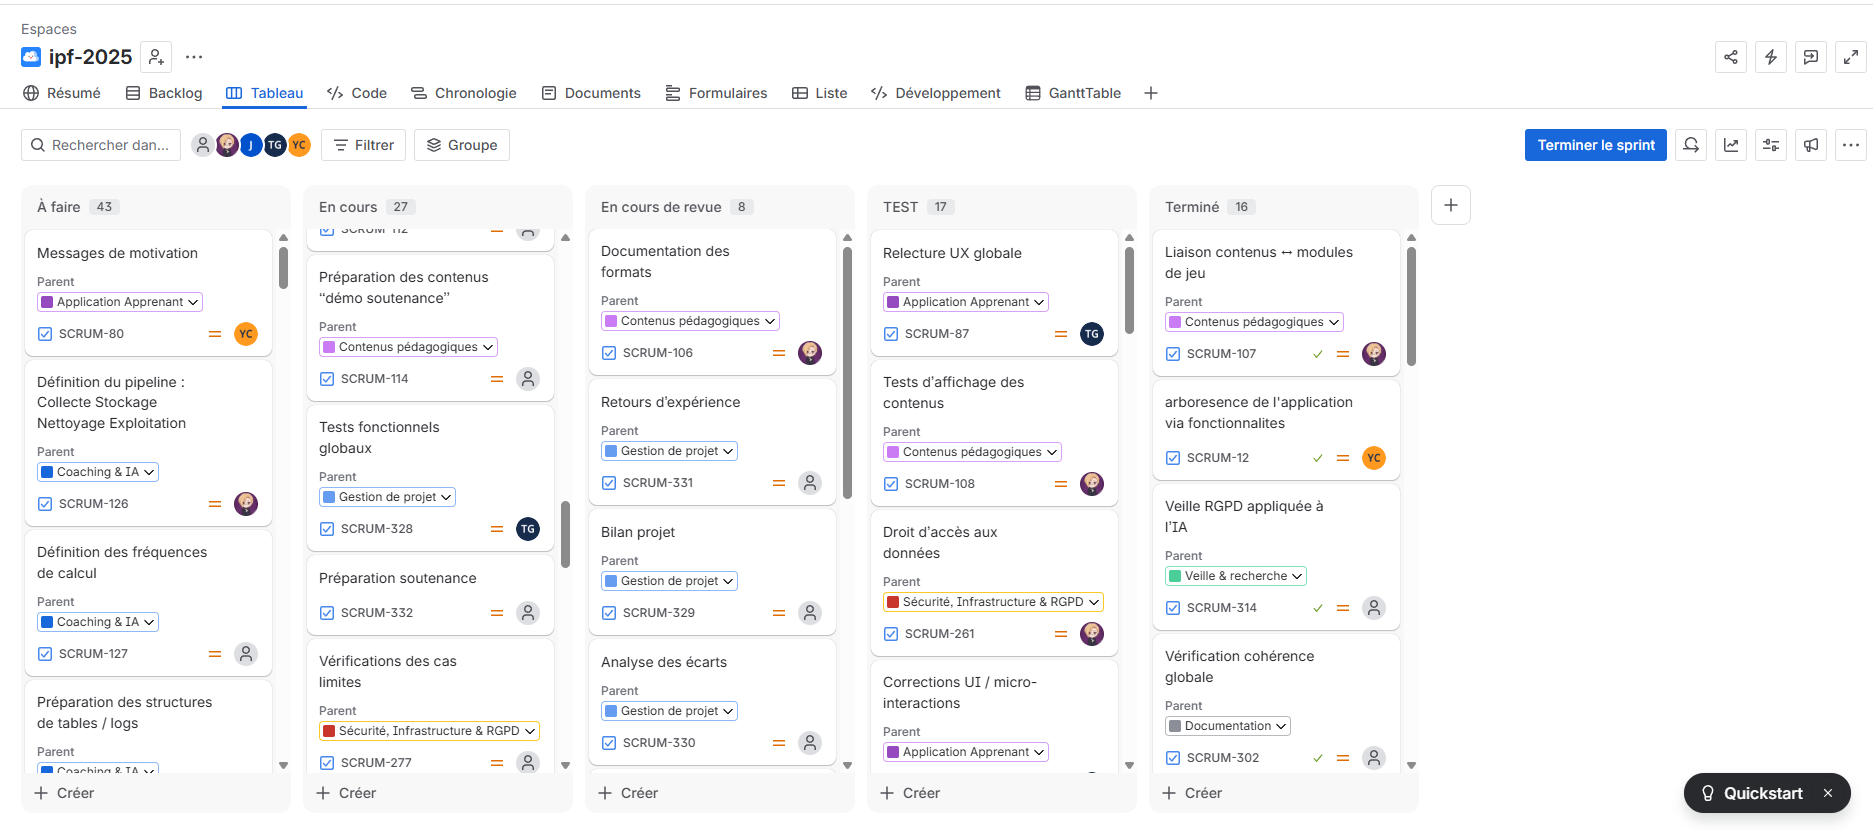
\includegraphics[width=\textwidth,height=0.25\textheight,keepaspectratio]{figures/ipf/jira-tabelau.png}\\[-0.05cm]
        {\footnotesize (b) Tableau Jira}
      \end{minipage}%
      \hfill
      \begin{minipage}[t]{0.49\textwidth}
        \centering
        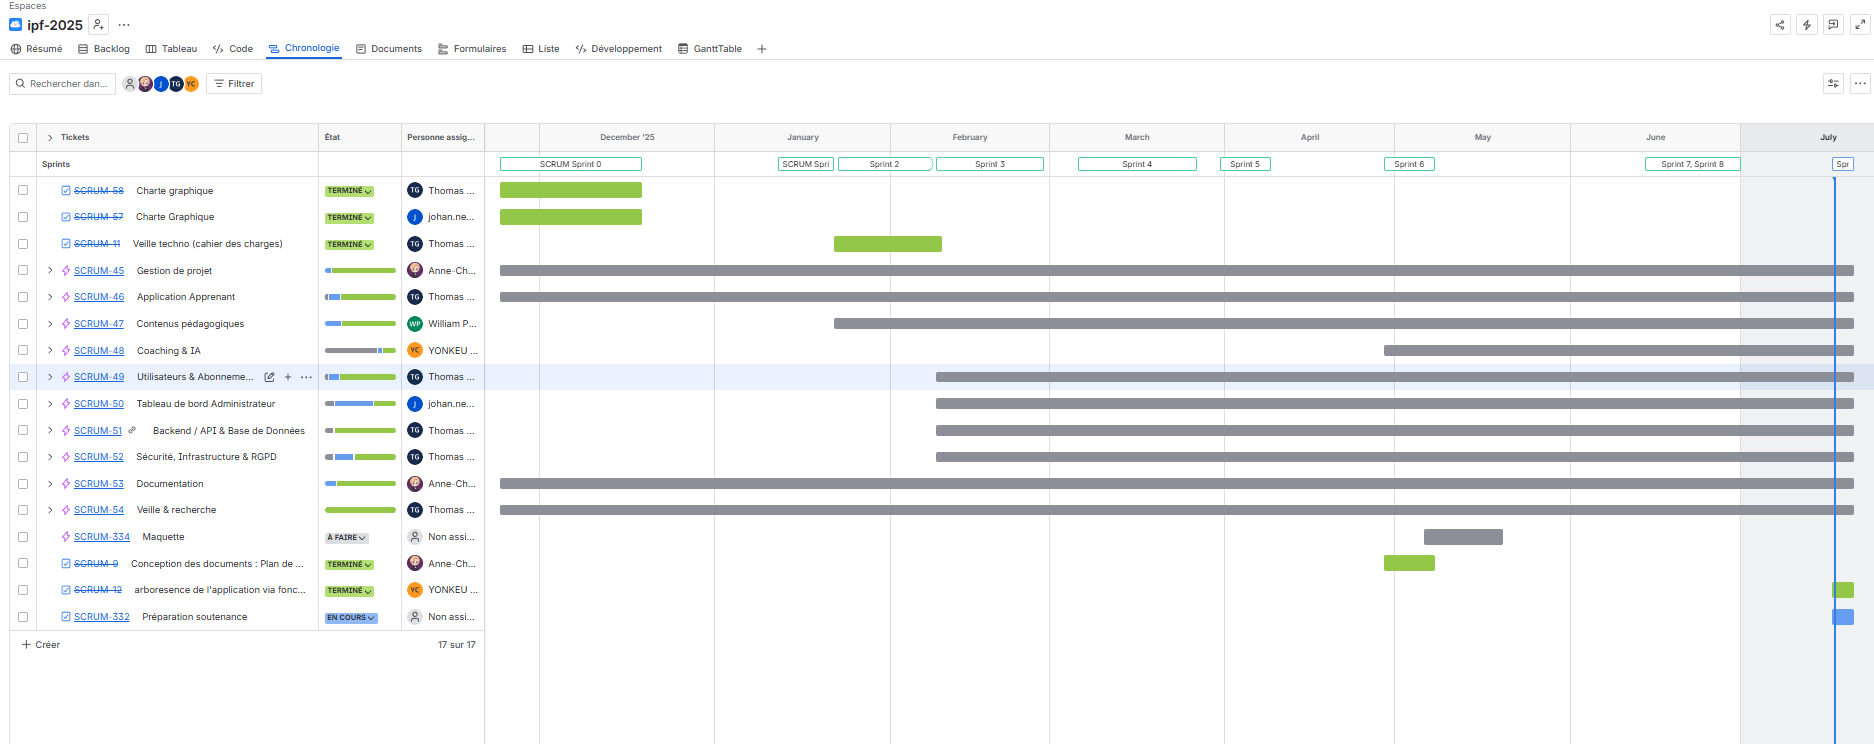
\includegraphics[width=\textwidth,height=0.25\textheight,keepaspectratio]{figures/ipf/jira-chonologie.png}\\[-0.05cm]
        {\footnotesize (c) Chronologie}
      \end{minipage}
    \end{minipage}%
  \or
    % Couverture des exigences fonctionnelles et non fonctionnelles.
    \begin{minipage}{\textwidth}
      \centering
      \begin{minipage}[t]{0.49\textwidth}
        \centering
        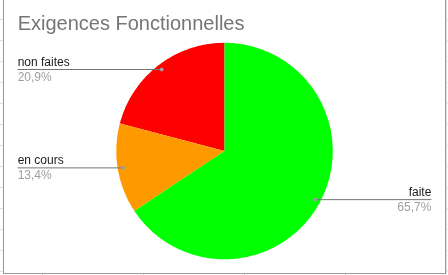
\includegraphics[width=\textwidth,height=0.13\textheight,keepaspectratio]{figures/ipf/vue_globale_avancement_exigence_1_functionnelles.png}\\[-0.05cm]
        {\scriptsize (a) Vue globale des exigences fonctionnelles}
      \end{minipage}%
      \hfill
      \begin{minipage}[t]{0.49\textwidth}
        \centering
        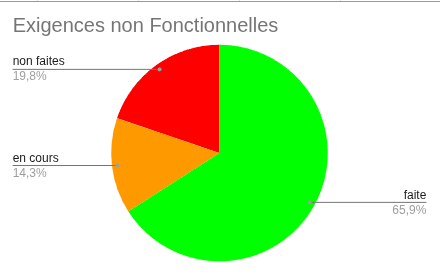
\includegraphics[width=\textwidth,height=0.13\textheight,keepaspectratio]{figures/ipf/vue_globale_avancement_exigence_2_non_functionnelles.png}\\[-0.05cm]
        {\scriptsize (b) Vue globale des exigences non fonctionnelles}
      \end{minipage}

      \vspace{0.16cm}

      \begin{minipage}[t]{0.49\textwidth}
        \centering
        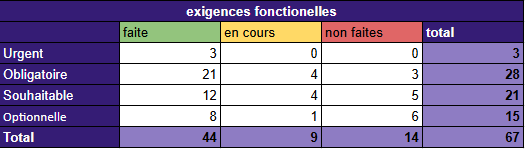
\includegraphics[width=\textwidth,height=0.13\textheight,keepaspectratio]{figures/ipf/synthese_exigence_fonctionnelles.png}\\[-0.05cm]
        {\scriptsize (c) Synthèse fonctionnelle}
      \end{minipage}%
      \hfill
      \begin{minipage}[t]{0.49\textwidth}
        \centering
        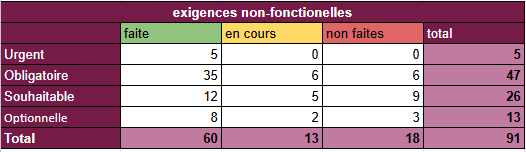
\includegraphics[width=\textwidth,height=0.13\textheight,keepaspectratio]{figures/ipf/synthese_exigence_non_fonctionnelles.png}\\[-0.05cm]
        {\scriptsize (d) Synthèse non fonctionnelle}
      \end{minipage}

      \vspace{0.16cm}

      \begin{minipage}[t]{0.49\textwidth}
        \centering
        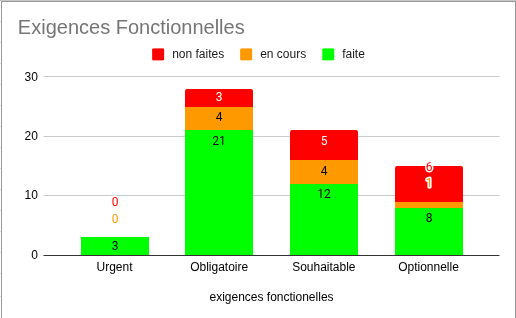
\includegraphics[width=\textwidth,height=0.13\textheight,keepaspectratio]{figures/ipf/exigences_functionneles_par_priorit__et_etat.png}\\[-0.05cm]
        {\scriptsize (e) Priorité et état des exigences fonctionnelles}
      \end{minipage}%
      \hfill
      \begin{minipage}[t]{0.49\textwidth}
        \centering
        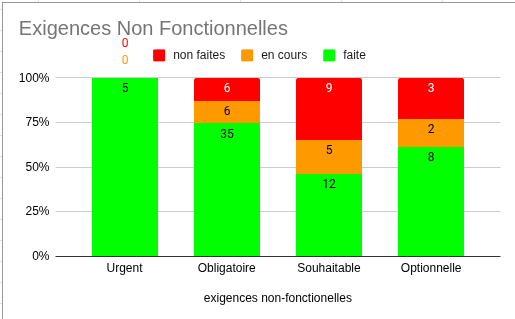
\includegraphics[width=\textwidth,height=0.13\textheight,keepaspectratio]{figures/ipf/exigences_non_functionneles_par_priorit__et_etat.png}\\[-0.05cm]
        {\scriptsize (f) Priorité et état des exigences non fonctionnelles}
      \end{minipage}

      \vspace{0.16cm}

      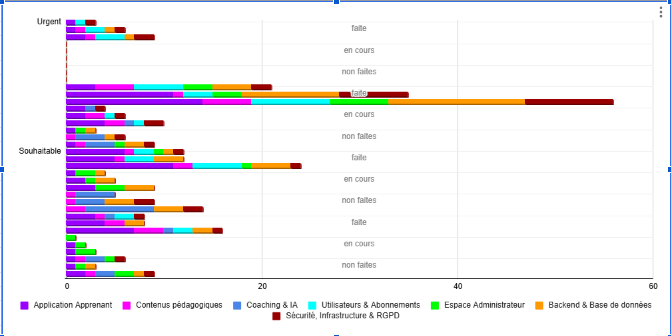
\includegraphics[width=\textwidth,height=0.15\textheight,keepaspectratio]{figures/ipf/repartition_sectorielle_exigences_par_priorite_etat.png}\\[-0.05cm]
      {\scriptsize (g) Répartition sectorielle des exigences par priorité et état}
    \end{minipage}%
  \or
    % Matrice de criticité des risques et règle d'escalade.
    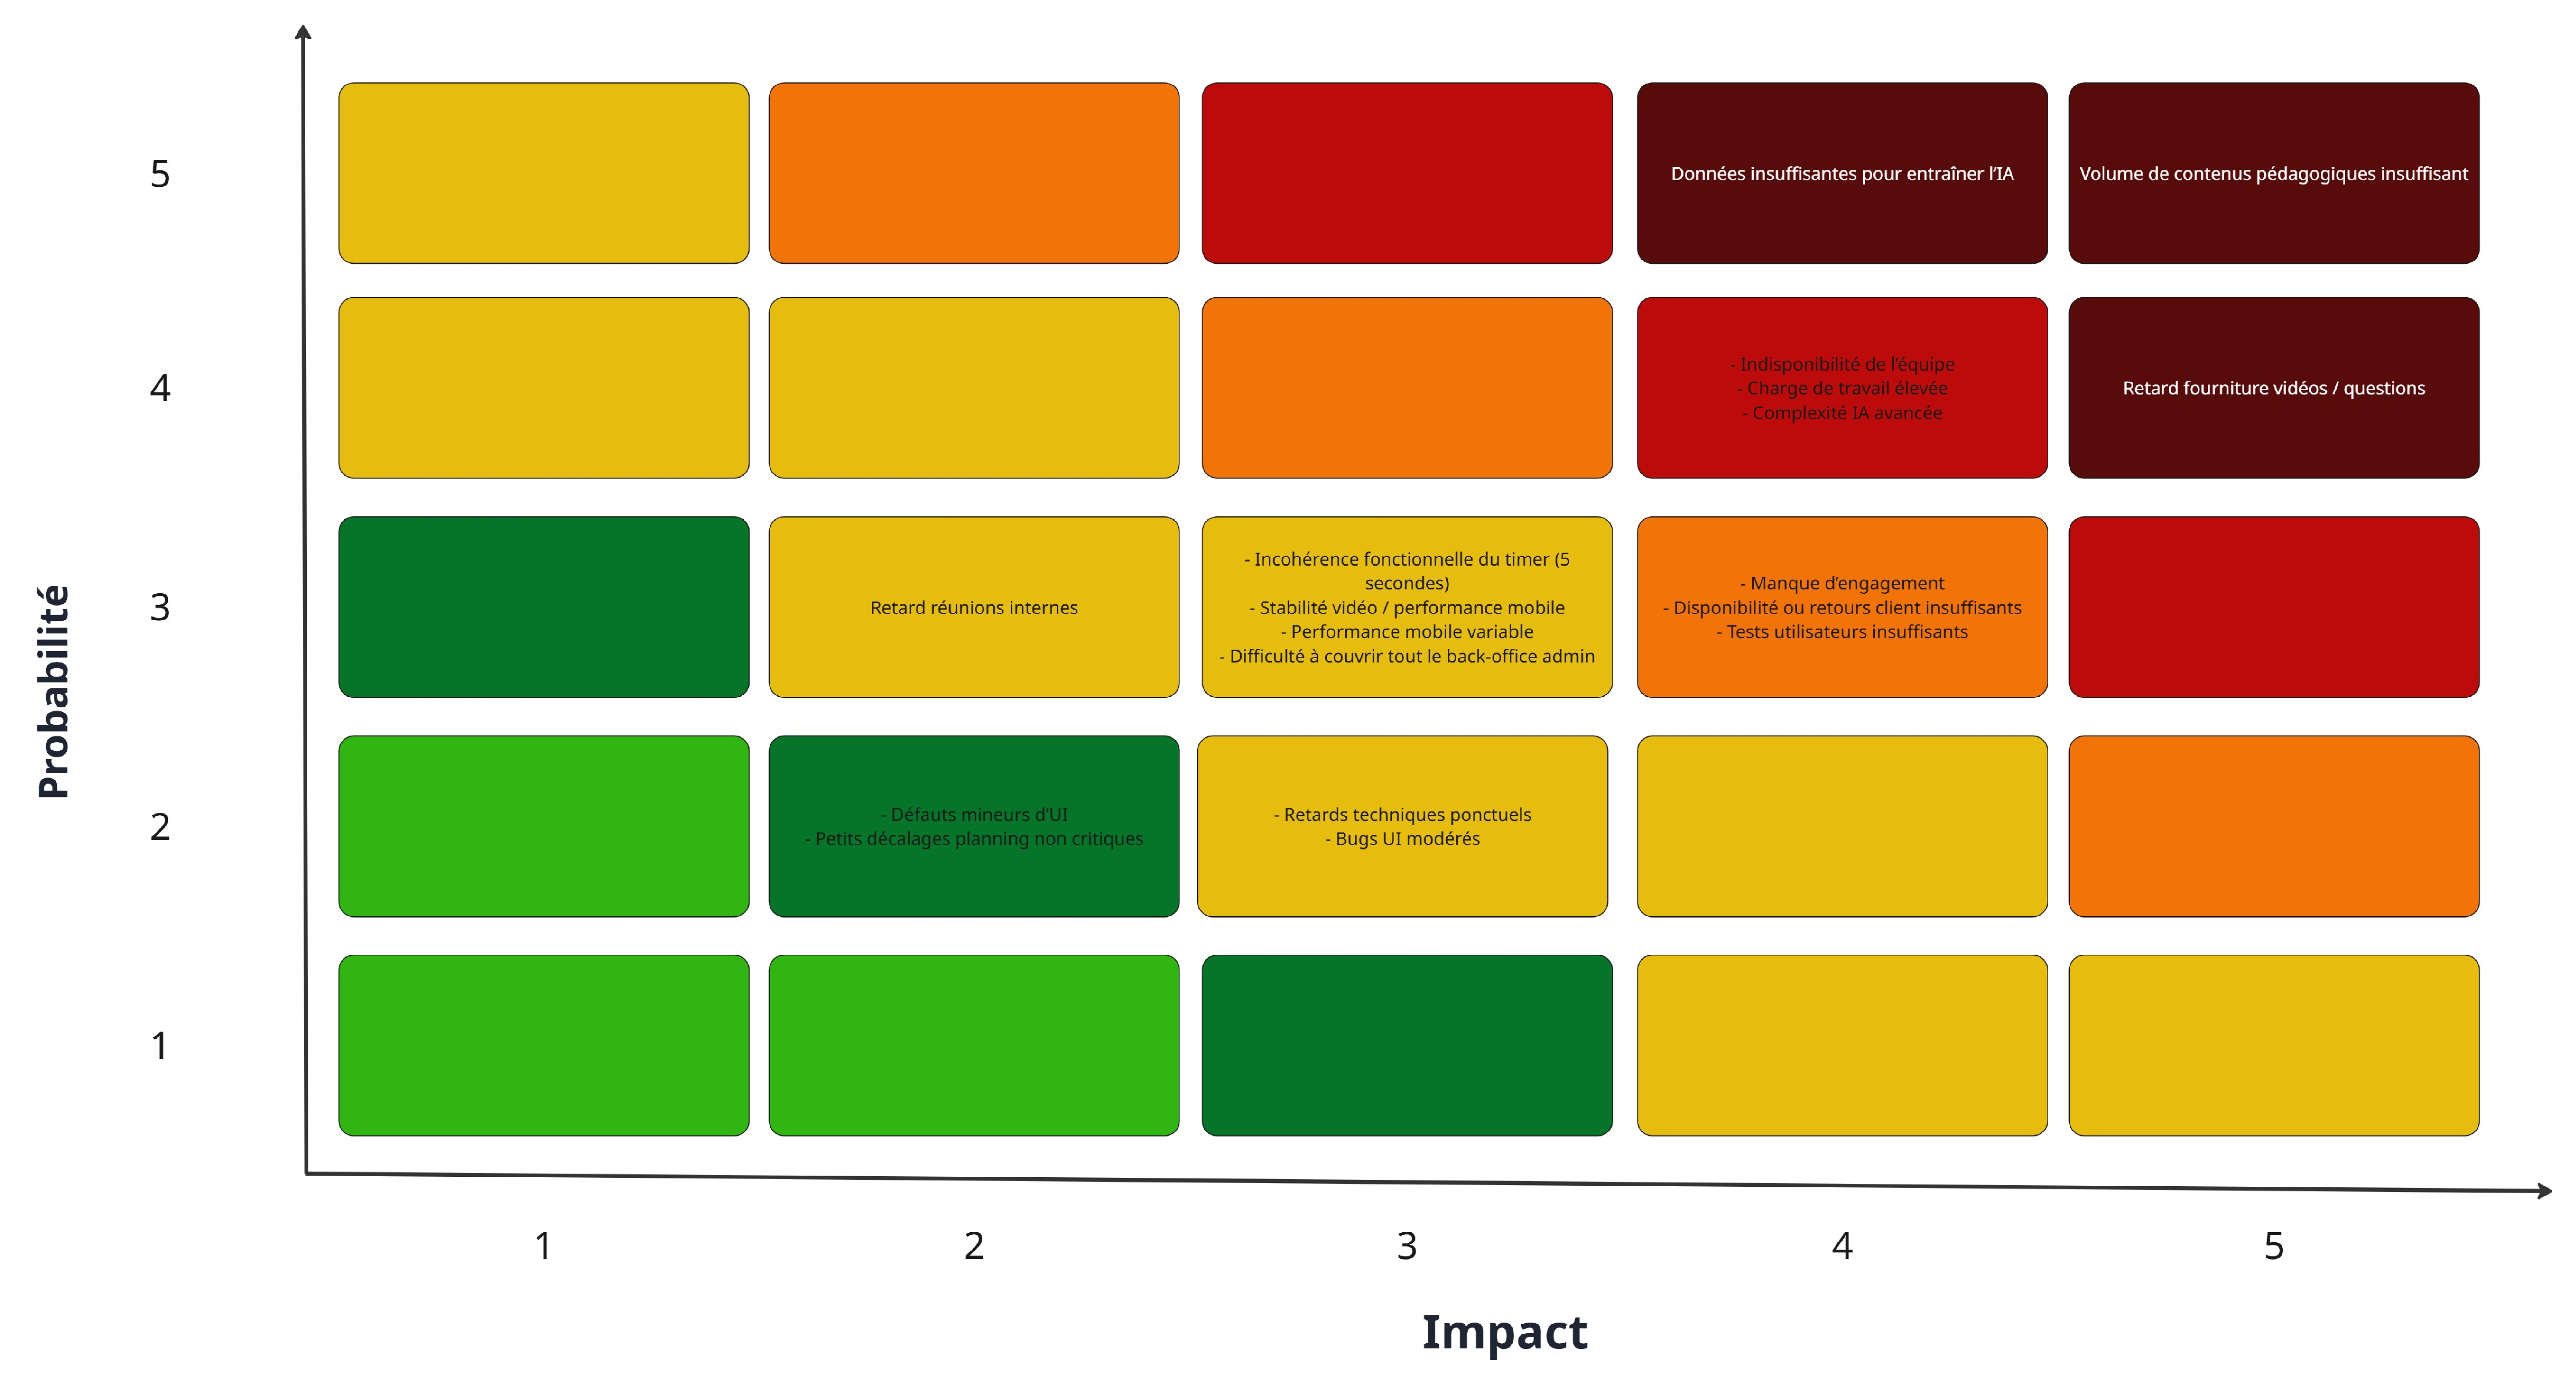
\includegraphics[width=\textwidth,height=0.56\textheight,keepaspectratio]{figures/ipf/matrice_risque-5sc.pdf}%
  \or
    % Plan de formation : tableau structuré fourni pour le dossier.
    \begin{minipage}{\textwidth}
      \centering
      \small
      \renewcommand{\arraystretch}{1.18}
      \begin{tabular}{p{3.0cm} p{3.1cm} p{7.2cm}}
        \toprule
        \textbf{Domaine} & \textbf{Outils / technologies} & \textbf{Objectif de montée en compétences} \\
        \midrule
        UX/UI et maquettage & Figma & Concevoir des maquettes compréhensibles, valider les parcours utilisateurs et fournir des supports exploitables pour le développement. \\
        Backend et base de données & Supabase / PostgreSQL & Comprendre la structure des données, l'authentification, les règles d'accès et la cohérence des informations stockées. \\
        Frontend administrateur & React / Vite & Développer une interface web dynamique permettant la gestion des contenus, des utilisateurs et des statistiques. \\
        Développement mobile & Flutter / Dart & Produire l'application apprenant, gérer les écrans, la navigation, les performances et l'intégration avec le backend. \\
        Gestion de projet & Jira / Confluence / Teams & Structurer les sprints, suivre les tâches, documenter les décisions, piloter les risques et répartir la charge. \\
        Déploiement et environnements & GitHub / Docker / Vercel / Stores mobiles & Comprendre la gestion des versions, les environnements, la livraison et les contraintes de publication. \\
        Conformité et sécurité & RGPD / Authentification / Paiements & Identifier les données sensibles, sécuriser les accès, limiter les risques et préparer une future mise en production. \\
        \bottomrule
      \end{tabular}
    \end{minipage}%
  \or
    % Documentation développeur MkDocs préparée pour la reprise.
    \begin{minipage}{\textwidth}
      \centering
      \begin{minipage}[t]{0.49\textwidth}
        \centering
        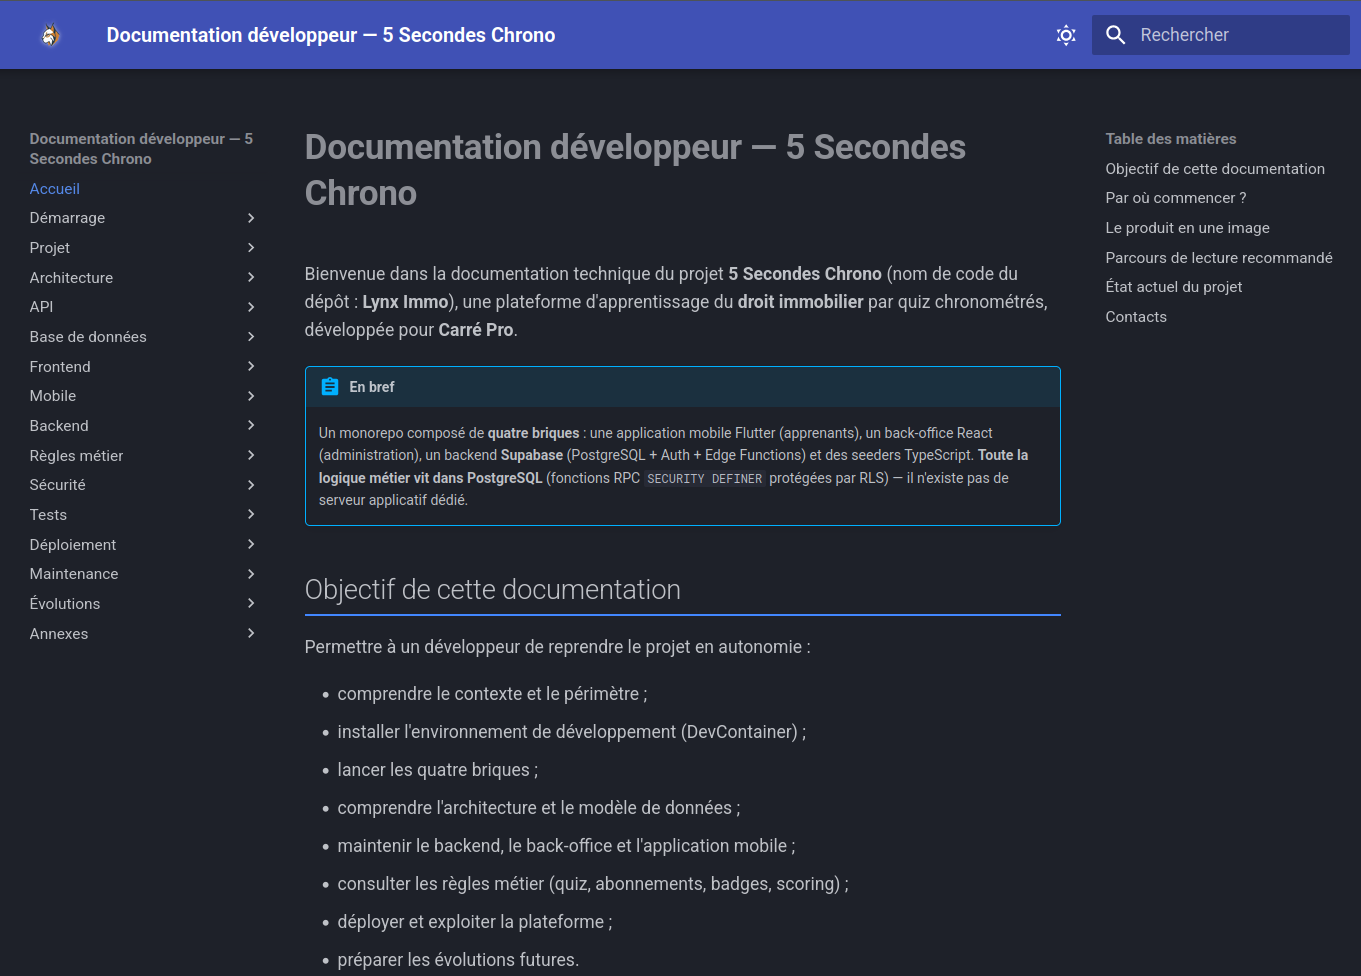
\includegraphics[width=\textwidth,height=0.36\textheight,keepaspectratio]{figures/ipf/acceuil_doc_dev_mkdocs.png}\\[-0.05cm]
        {\footnotesize (a) Accueil et arborescence de la documentation}
      \end{minipage}%
      \hfill
      \begin{minipage}[t]{0.49\textwidth}
        \centering
        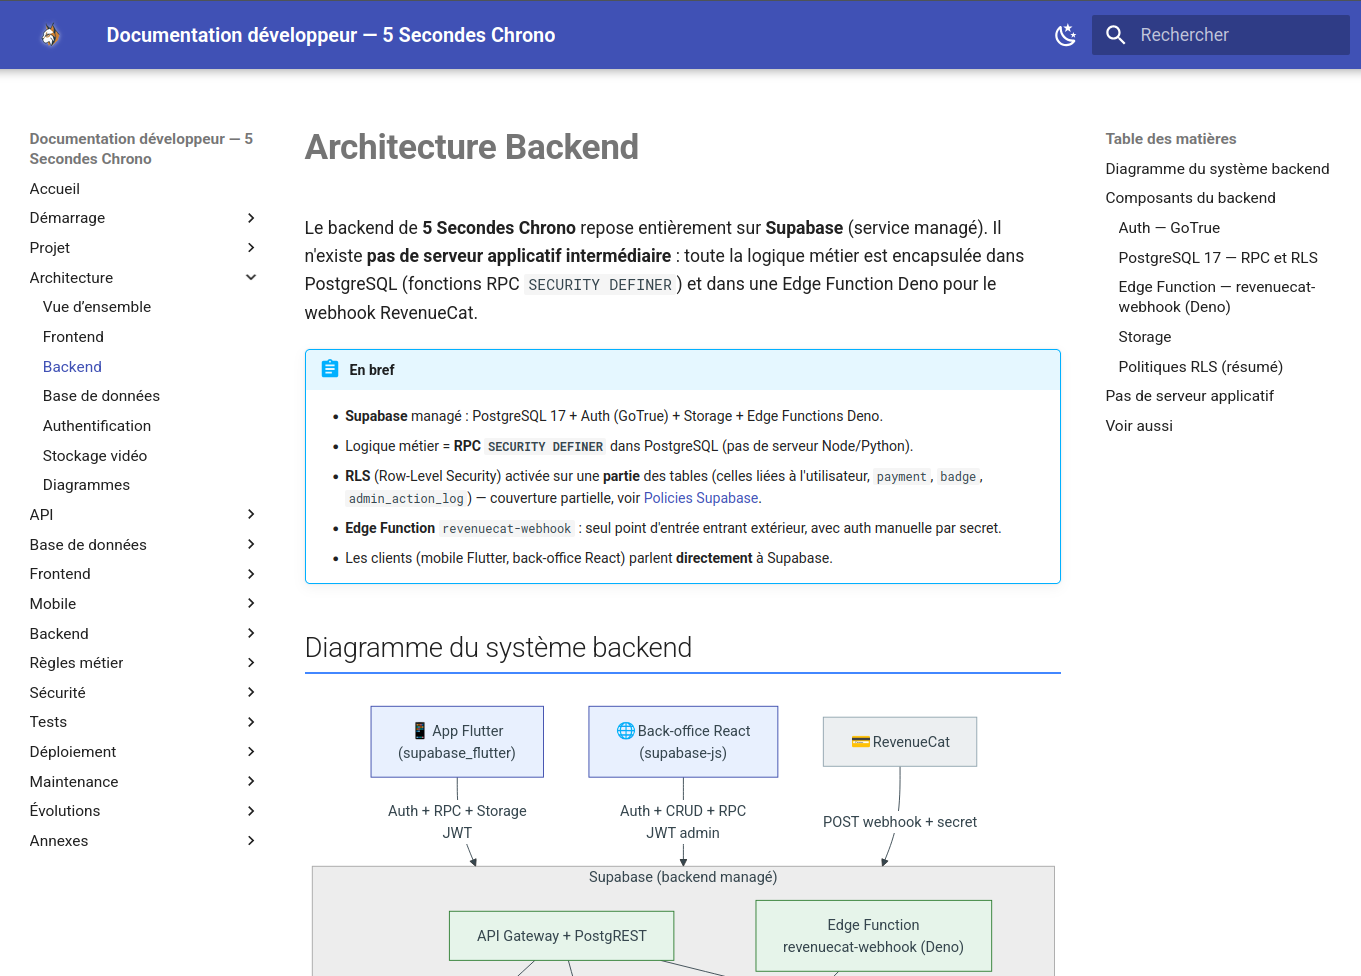
\includegraphics[width=\textwidth,height=0.36\textheight,keepaspectratio]{figures/ipf/exemple_page_doc_mkdocs.png}\\[-0.05cm]
        {\footnotesize (b) Exemple de page technique}
      \end{minipage}
    \end{minipage}%
  \else
    \PackageError{lynx-figures}{Nombre de placeholders Lynx Immo inattendu}{Le chapitre Lynx Immo contient plus de 11 appels a \string\fbox.}%
  \fi
}
